% As per supervisor feedback, no longer making this its own chapter
% \chapter{What you did}
% \label{ch:whatYouDid}


% \engExpl{Choose your own chapter title to describe this}
% \sweExpl{[Vad gjorde du? Hur gick det till? – Välj lämplig rubrik (“Genomförande”, “Konstruktion”, ”Utveckling”  eller annat]}


% \engExpl{What have you done? How did you do it? What design decisions did you make? How did what you did help you to meet your goals?}
% \sweExpl{Vad du har gjort? Hur gjorde du det? Vilka designval gjorde du?\\
% Hur kom det du hjälpte dig att uppnå dina mål?}


% the following sets the TOC entry to break after the & - note you have to include the first letter of the following word as it get swolled by the \texorpdfstring{}{} processing


% \section[Hardware/Software design …/Model/Simulation model \&\texorpdfstring{\\}{ p} parameters/…]{Hardware/Software design …/Model/Simulation model \& parameters/…}


\section{Proof of Concepts}


The following section will outline the various \gls{POC} applications that were built before the actual software that was written to conduct the research outlined in this thesis. Even though it’s difficult to distinctly separate \gls{POC}s from each other, in total around 9 \gls{POC}s were produced. Each \gls{POC} will outline what it was trying to accomplish and what the outcome was. Some \gls{POC}s have been omitted since they were either dead-ends, or simply too similar to one of the other \gls{POC}s described below.


\subsection{Langchain based applications}


Langchain is a company \footnote{\href{https://langchain.com}{langchain.com} (accessed on \today)} and framework \footnote{\href{https://python.langchain.com}{python.langchain.com} (accessed on \today)} for building context aware reasoning applications. The framework allows for easy composition of language models and \gls{RAG} techniques and tools that makes it easy to build chatbots with a connected knowledge base. This section outlines some \gls{POC}s that were made with the langchain framework.


\subsubsection{GPT-4 and text-embedding-3-large}
\label{sec:poc_gpt_langchain}


To build a chat application with an AI-assistant that has access to an external knowledge base, one of the most popular approaches is to use langchain to connect the following four parts.


\begin{enumerate}
        \item A \gls{LLM}, such as GPT-4 to run the chat.
        \item A \gls{LLM}, such as GPT-4 to run the query construction.
        \item An embedding function, such as OpenAI’s text-embedding-3-large used to index and query documents.
        \item A vector store, such as ChromaDB, that stores the vector embeddings and associated documents \footnote{\href{https://www.trychroma.com/}{trychroma.com/} (accessed on \today)}
\end{enumerate}.


In this configuration, Lanchain acts as the glue connecting these components and handling tasks like chunking larger documents. The goal of this \gls{POC} was to test a common approach for building AI assistants and evaluate its potential for use in the full study. \href{https://www.youtube.com/watch?v=bKjxi-NKRHo}{A video can be seen here} that showcases this \gls{POC}.


\subsubsection{Mistral 7B v0.2 and e5-large-v2}


There was a \gls{POC} constructed that had the same approach as the one outlined in \ref{sec:poc_gpt_langchain} with the notable requirement that all tools had to be under an open source licence. This meant the GPT-4 model and text-embedding-3-large models couldn’t be used. A similar version of the same \gls{POC} was made that used the Mistral 7B v0.2 model and the embedding function e5-large-v2 \cite{wang_text_2024}. These are both under an open source licence and are freely available on Huggingface \footnote{\href{https://huggingface.co/mistralai/Mistral-7B-Instruct-v0.2}{huggingface.co/mistralai/Mistral-7B-Instruct-v0.2} (accessed on \today)} \footnote{\href{https://huggingface.co/intfloat/e5-large-v2}{huggingface.co/intfloat/e5-large-v2} (accessed on \today)}. This \gls{POC} did however suffer from poor performance in initial tests for retrieval and performance. It was difficult to tune the prompts to get decent performance. This \gls{POC} showed it was difficult for the researcher to get good performance out of certain models using the langchain framework.


\subsection{Custom applications}


This section outlines some major and minor \gls{POC}s that were made without any frameworks that are popular \gls{LLM} applications, aside from very common python libraries such as pytorch and hugginface’s transformers library.


\subsubsection{Simple Python API for models on Huggingface}


Langchain and similar tools support running language models locally. However, working with the prompt templates in less advanced models than GPT-4 and achieving good retrieval and chat performance was challenging. Therefore, a simple \gls{POC} was developed to create higher-level Python abstraction APIs on top of the Hugging Face Transformers library that could be integrated into completely custom solutions. These APIs include examples like those shown in listings ~\ref{fig:python-apis-for-llm} and ~\ref{fig:python-apis-for-embeddings}. A short video \href{https://www.youtube.com/watch?v=VG16oWK_LUQ}{can be seen here} that demonstrates a chat application (without an integrated knowledge base) built on-top of these simple APIs.


\begin{listing}[H]
\centering
\renewcommand{\theFancyVerbLine}{\scriptsize\arabic{FancyVerbLine}}
\scriptsize
\begin{minted}[
frame=lines,
framesep=2mm,
baselinestretch=1.2,
fontsize=\scriptsize,
linenos
]{python}
def load_hf_model(
    model_path: str,
    device: str
) -> (transformers.AutoModelForCausalLM, transformers.AutoTokenizer):
    """
    Loads a Hugging Face causal language model and its tokenizer for a given
    model path and device.
    """

def generate_text(
    model: transformers.AutoModelForCausalLM,
    tokenizer: transformers.AutoTokenizer,
    device: str,
    params: Params,
    prompt: str
) -> str:
    """
    Generates text from a prompt using the specified model, tokenizer, and
    generation parameters.
    """

async def generate_text_streaming(
    model: transformers.AutoModelForCausalLM,
    tokenizer: transformers.AutoTokenizer,
    device: str,
    params: Params,
    prompt: str
) -> AsyncGenerator[str, None]:
    """
    Asynchronously generates text from a prompt, yielding tokens incrementally.
    Useful for streaming responses.
    """

def _tokenise_inputs(
    tokeniser: transformers.AutoTokenizer,
    input_texts: list[str],
    max_length: int = 8192
) -> dict:
    """
    Tokenizes the input texts with padding and truncation.
    """

def should_stop_generating(
    output_token_ids: list,
    tokenizer: transformers.AutoTokenizer,
    params: Params,
    token_id: int
) -> bool:
    """
    Determines whether to stop generating text based on stop conditions.
    """
\end{minted}
\caption{High level API on-top of Huggingface's tranformers library that can be used for generating text using models available on Huggingface.}
\label{fig:python-apis-for-llm}
\end{listing}

\begin{listing}[H]
\centering
\renewcommand{\theFancyVerbLine}{\scriptsize\arabic{FancyVerbLine}}
\scriptsize
\begin{minted}[
frame=lines,
framesep=2mm,
baselinestretch=1.2,
fontsize=\scriptsize,
linenos
]{python}
def load_hf_embedding_model(
    model_path: str,
    device: str
) -> (torch.nn.Module, transformers.AutoTokenizer):
    """
    Loads a Hugging Face embedding model and its tokenizer for a given model
    path and device.
    """

async def compute_embedding(
    model: torch.nn.Module,
    tokeniser: transformers.AutoTokenizer,
    text: str
) -> List[float]:
    """
    Computes and returns the normalized embedding for a given text using the
    specified model and tokenizer.
    """

def _compute_model_embeddings(
    model: torch.nn.Module,
    tokenised_inputs: dict
) -> torch.Tensor:
    """
    Computes the model embeddings from the tokenized inputs.
    """
\end{minted}
\caption{High level API on-top of Huggingface's tranformers library that can be used for generating vector embeddings using models available on Huggingface.}
\label{fig:python-apis-for-embeddings}
\end{listing}



\subsubsection{Mistral 7B v0.2 and Opensearch}


The goal with this \gls{POC} was to build a version of the \gls{RAG} application that didn’t use a vector embedding function. Instead, this \gls{POC} would utilise a traditional search service such as Elasticsearch or Opensearch. These implement "traditional" search algorithms such as \gls{TF-IDF}, as outlined in section \ref{sec:background_tfidf}. This \gls{POC} was very easy to implement and showed great promise.


\subsubsection{Post processing for smaller models}
\label{sec:post_processing}


When working with models that don’t produce the best scores on public benchmarks, such as \gls{MMLU}, there are a number of techniques that can be employed that could improve the performance of a \gls{RAG} system. These generally smaller models suffer from worse scores on precision and recall benchmarks. This means they are worse at recalling facts injected into the conversation by a \gls{RAG} pipeline. One of the techniques that can be used is post-processing retrieved documents before they are inserted into the chat. There are a number of ways of achieving this. One of the techniques that was tried, and eventually implemented in the final study, was to use a post-processing mechanism, where each of the retrieved documents are passed through a post-processing function, which reduce the size of the document, as shown in \autoref{eq:without_post_processing} and \autoref{eq:with_post_processing}.


\begin{equation}
R = \text{LLM}\left(Q, \{D_i\}_{i=1}^N\right)
\label{eq:without_post_processing}
\end{equation}


Where:
\begin{itemize}
        \item \( R \) is the generated response.
        \item \( \text{LLM} \) is the language model function.
        \item \( Q \) is the user query.
        \item \( \{D_i\}_{i=1}^N \) are the matching documents retrieved from the index.
\end{itemize}


\begin{equation}
R = \text{LLM}\left(Q, \{\text{PP}(D_i, P)\}_{i=1}^N\right)
\label{eq:with_post_processing}
\end{equation}


Where:
\begin{itemize}
        \item \( \text{PP} \) is the post-processing function.
        \item \( P \) is the post-processing prompt.
\end{itemize}


There are different strategies for the prompt that reduce the size of the document. This prompt can instruct the language model to extract quotes from the document related to the query, summarise key facts related to the query, or a number of other methods. The one that was chosen for the final study was extracting quotes as this showed the most potential. \autoref{fig:without_post_processing} and \autoref{fig:with_post_processing} illustrate this process.


% https://lucid.app/lucidchart/7d7e52da-e0c5-45de-9d50-6fc1313b1528/edit

\begin{figure}[H]
    \centering
    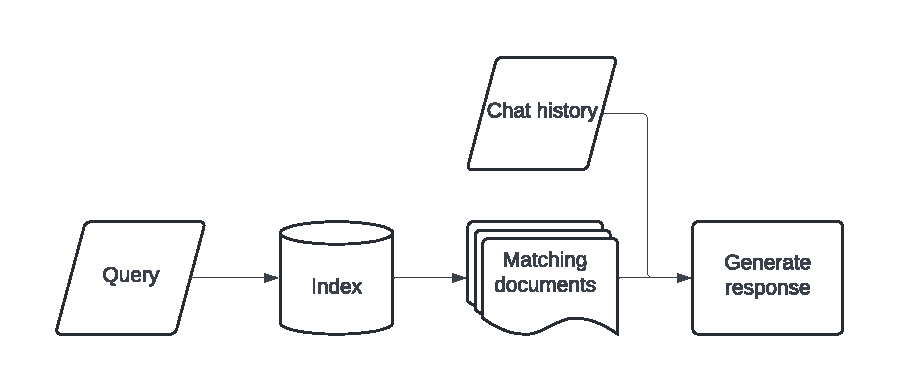
\includegraphics[width=\textwidth]{content/figures/assets/10-without-post-processing.pdf}
    \caption{Diagram that shows how documents are injected into the chat, without post-processing}
    \label{fig:without_post_processing}
\end{figure}



% https://lucid.app/lucidchart/f126e1c6-7c22-4445-8977-d2e8ccfba351/edit

\begin{figure}[H]
    \centering
    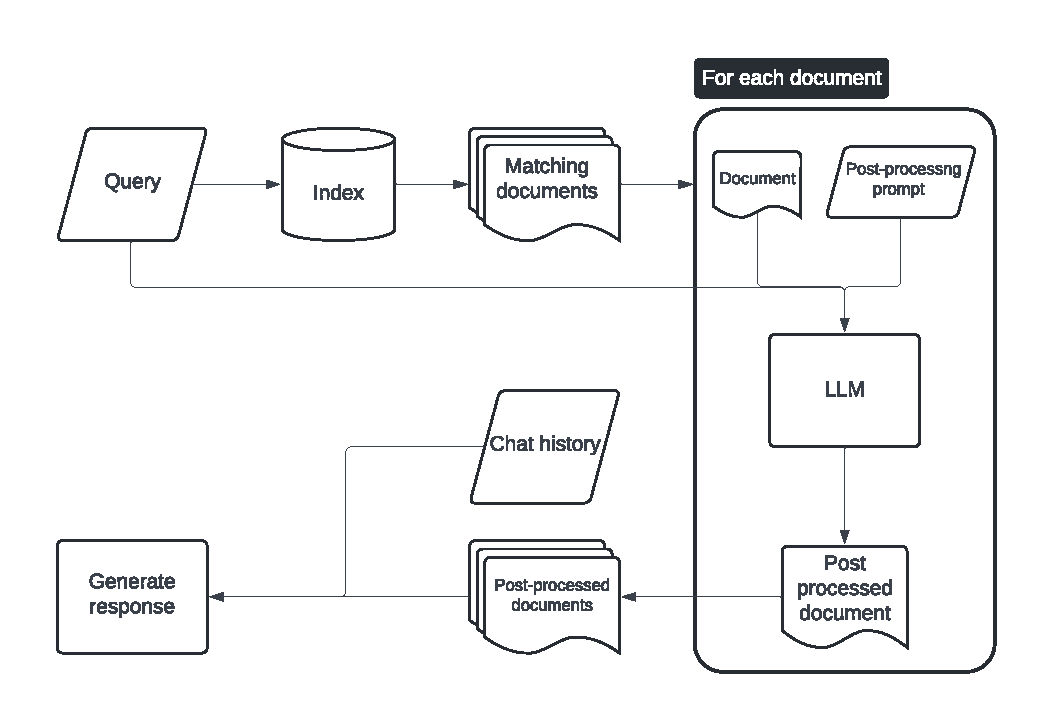
\includegraphics[width=\textwidth]{content/figures/assets/11-with-processing.pdf}
    \caption{Diagram that shows how documents are post-processed before they are injected into the chat}
    \label{fig:with_post_processing}
\end{figure}



\subsubsection{Too much processing}


Processing the documents to be smaller in size such that smaller models could accurately recall facts from retrieved documents was investigated until the point where additional processing would no longer improve the quality of the answers,


There were additional efforts put towards investigating the processing of documents to be smaller in size. The goal was to enable smaller models to accurately recall facts from the retrieved documents. This process continued until additional processing no longer improved the quality of the answers. There were \gls{POC}s produced that for instance processed the documents during the indexing phase in addition to the retrieval phase. During the indexing the documents were compiled into smaller "facts" that were indexed on their own. However, reducing the documents in size decreased the retrieval algorithms, both \gls{TF-IDF} algorithms and embedding functions.


Some processing however could improve the performance. Such as including a summary of the entire document with each chunk of that document. In summary, pre-processing the documents, and chunks of each document, during the indexing process, did increase the system’s ability to produce accurate answers to user queries. However, processing the documents too much was found to eventually lead to a reduction in accuracy.


\section{The architecture of the software}


This section will outline the final software that was constructed to investigate the research question in this thesis. The section will describe the goal of the software, what components it consists of, how each component works and showcase how it helps students get answers to their questions.


\subsection{What the purpose of the software is}


The purpose of the software is to crawl canvas course rooms and index their data into a knowledge base. The software should expose this knowledge base in a chat based application integrated into the same course room it has crawled. The tool should be able to randomly sample a configuration of models and tools for indexing, retrieval and chat between users of the tool. Finally, the tool should inject questions into the chat and track the necessary data points to investigate the research question of this thesis outlined in section~\ref{sec:researchQuestion}.


\subsection{What the software can test}


The software was constructed to measure how certain variables would impact the user feedback to certain configured questions. Section~\ref{sec:survey_questions_injected_into_the_chat} shows all questions that were used, and what possible answers existed. The variables that were supported can be seen in \autoref{tab:models_supported}, \autoref{tab:indicies_supported} and \autoref{tab:indicies_supported_with_postprocessing}. The table also includes a column if this variable was actually used in the experiment, or if it was just implemented but never enabled in the experiments.


\begin{table}[H]
\centering
{\footnotesize
\begin{tabularx}{\textwidth}{@{}Xcc@{}}
\toprule
\textbf{Variable} & \textbf{Supported} & \textbf{Enabled} \\ \midrule
\textit{GPT-4} by \textit{OpenAI}              & Yes & Yes \\
\textit{Mistral 7B Instruct v0.2} by \textit{MistralAI} & Yes & Yes \\
\textit{Llama 3 8B Instruct} by \textit{Meta} & Yes & No  \\
\bottomrule
\end{tabularx}
}
\vspace{2mm}
\caption{The models supported by the software and if they were used in the study}
\label{tab:models_supported}
\end{table}


\begin{table}[H]
\centering
{\footnotesize
\begin{tabularx}{\textwidth}{@{}Xcc@{}}
\toprule
\textbf{Variable} & \textbf{Supported} & \textbf{Enabled} \\ \midrule
Full text search              & Yes & No \\
Vector search using \textit{SFR Embedding Mistral} by \textit{Salesforce}              & Yes & No \\
Vector search using \textit{text-embedding-3-large} by \textit{OpenAI}              & Yes & Yes \\
\bottomrule
\end{tabularx}
}
\vspace{2mm}
\caption{The indices supported by the software and if they were used in the study}
\label{tab:indicies_supported}
\end{table}


\begin{table}[H]
\centering
{\footnotesize
\begin{tabularx}{\textwidth}{@{}Xcc@{}}
\toprule
\textbf{Variable} & \textbf{Supported} & \textbf{Enabled} \\ \midrule
Full text search              & Yes & No \\
Vector search using \textit{SFR Embedding Mistral} by \textit{Salesforce}              & Yes & No \\
Vector search using \textit{text-embedding-3-large} by \textit{OpenAI}              & Yes & No \\
\bottomrule
\end{tabularx}
}
\vspace{2mm}
\caption{The indices supported by the software \textbf{with} post-processing enabled, and if they were used in the study}
\label{tab:indicies_supported_with_postprocessing}
\end{table}



\subsection{Overall architecture}


The software is primarily written in python, with a service-based architecture. This means it is divided into distinct domain specific services, each handling specific domains and functionalities. These services handle one of four things, \gls{LLM}-, Download-, Index- or Chat-functionality.


These services are written in such a way that they can be incorporated into any executable within the project. There are numerous executables within the application, these are;


\begin{itemize}
        \item A graphical user interface, which is a web-based application
        \item A HTTP rest API
        \item A websocket server
        \item A job-runner that execute background tasks from a queue
        \item A worker node for the \gls{LLM} service that keep a \gls{LLM} in-memory ready to generate a response to a prompt for the given model
\end{itemize}


\autoref{fig:system_architecture_diagram} shows an overview of the architecture of the software written to conduct the research and which components are called by other components.


% https://lucid.app/lucidchart/f5dc4477-fa25-44e8-93d9-946def9cd4a9/edit

\begin{figure}[H]
    \centering
    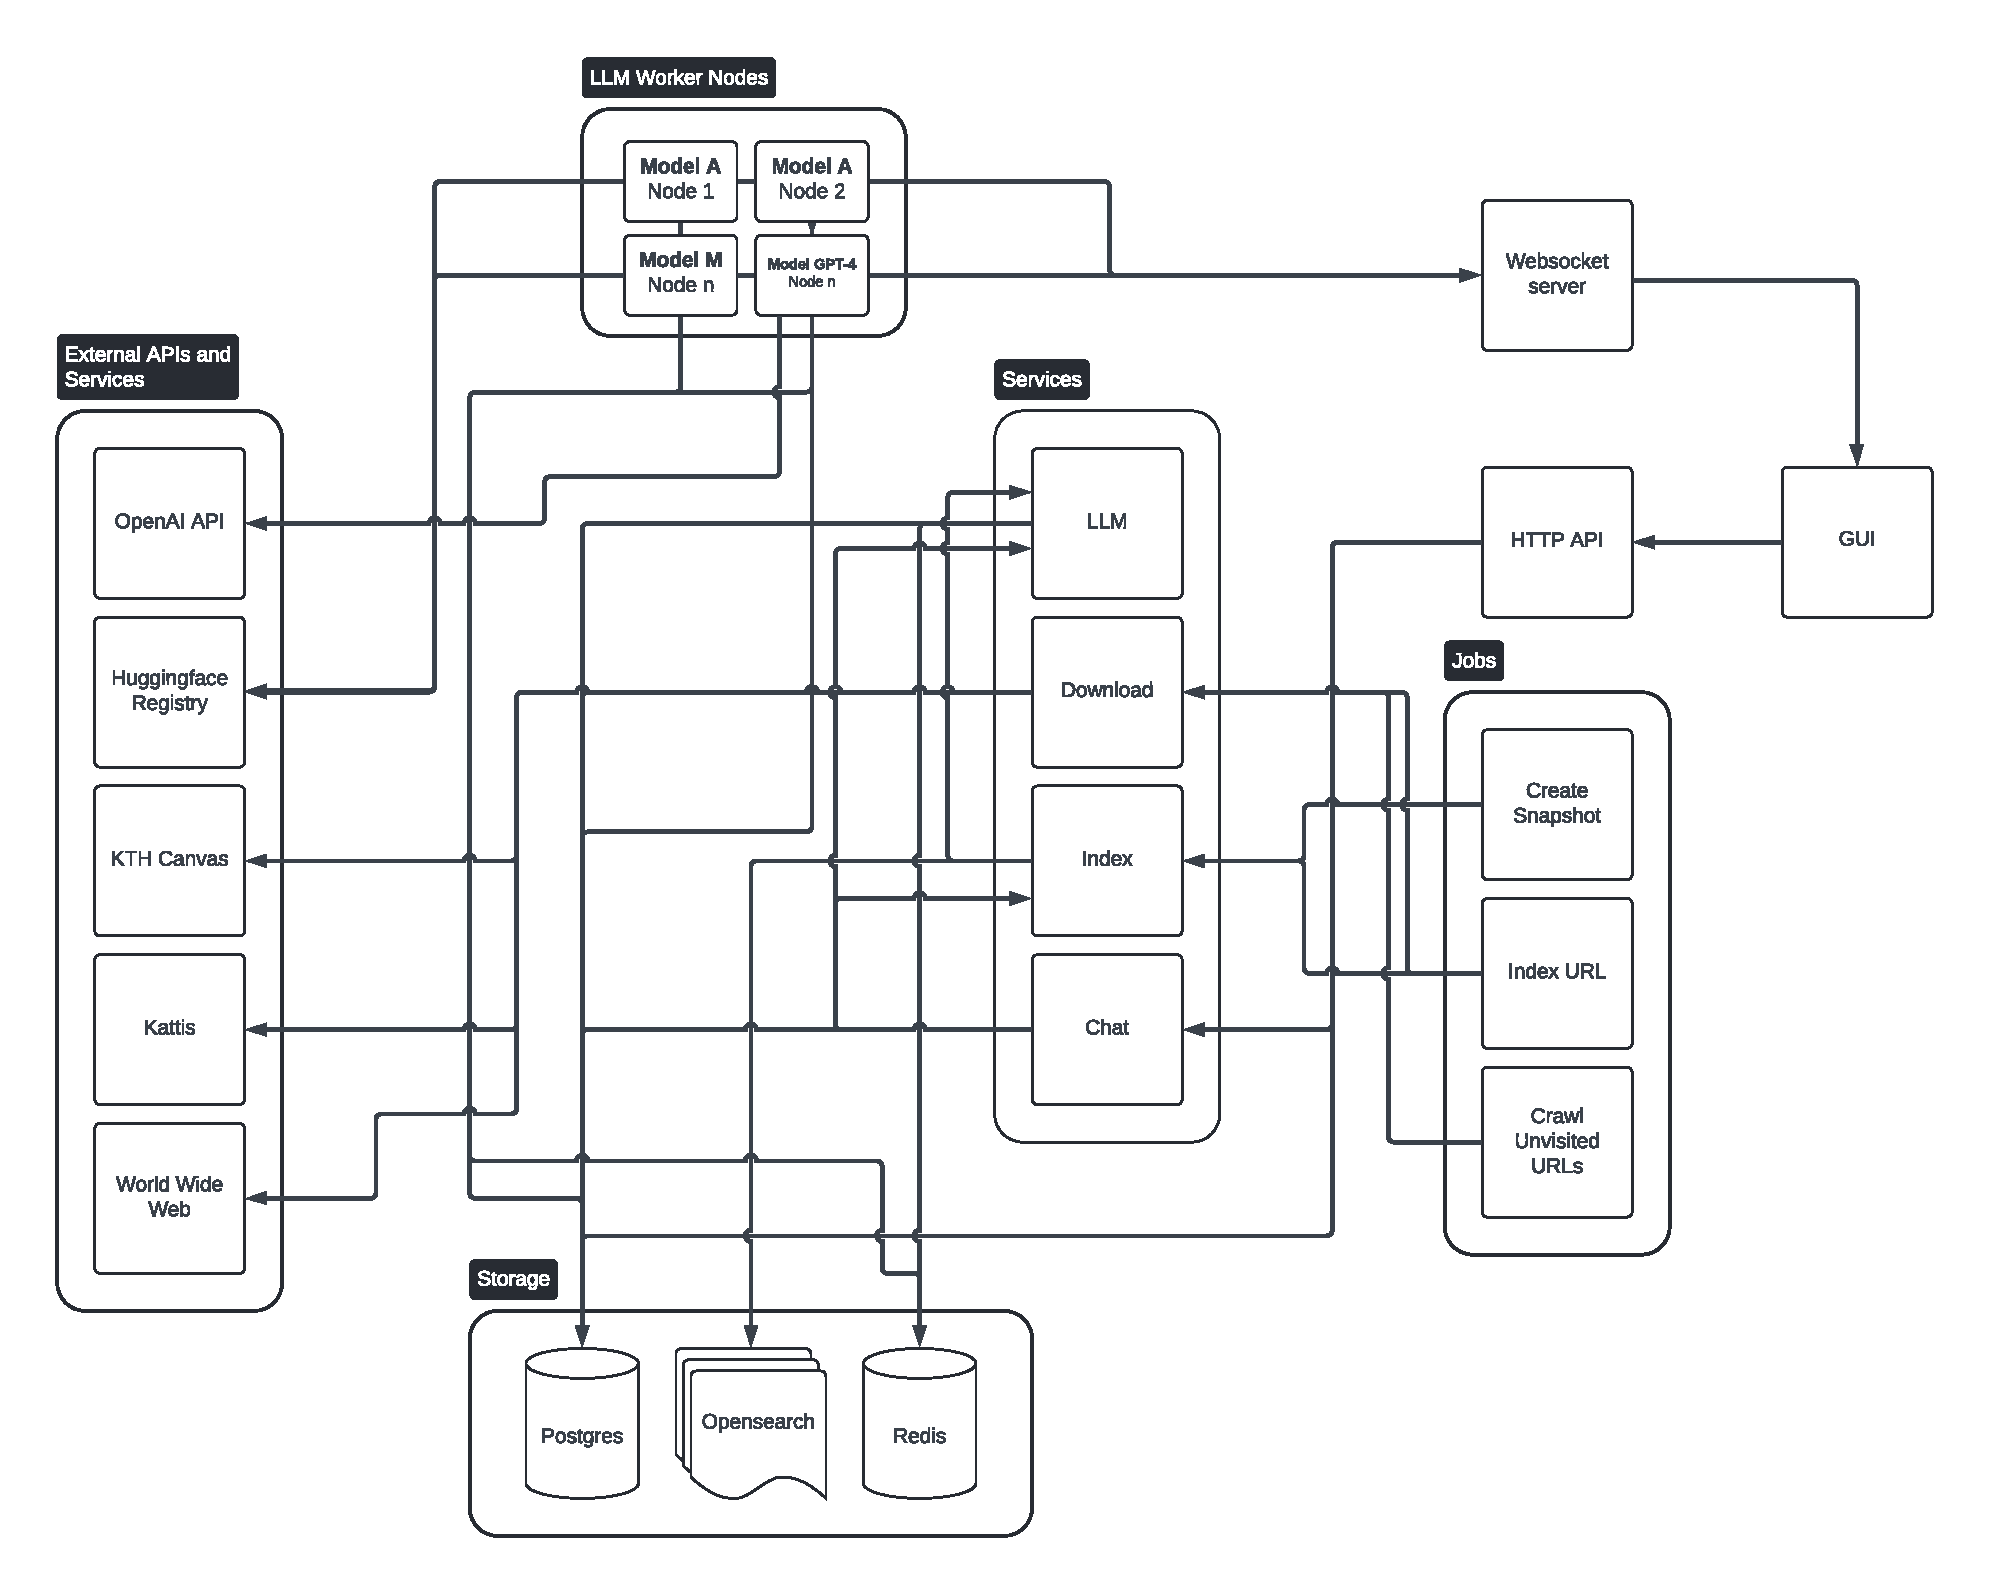
\includegraphics[width=\textwidth]{content/figures/assets/06-system-architecture-diagram.pdf}
    \caption{Diagram that shows the system architecture of the software constructed to run the study}
    \label{fig:system_architecture_diagram}
\end{figure}



\subsection{Dependencies}


The software is written on-top of numerous python and javascript libraries, these are documented in their entirety in the systems source code repository. In addition, the software needs the following major dependencies to operate.


\begin{itemize}
        \item A postgres database
        \item A opensearch index
        \item A redis in-memory storage
\end{itemize}


\subsection{Courseroom Crawler}


The software contains a job that is run every minute, which checks if a new snapshot should be taken of a course room. A snapshot contains all urls and their content that was crawled from a course room. A piece of content may be a canvas webpage, a file hosted on canvas, an external url or file etc.


If a new snapshot is created of a course room the crawler will immediately crawl the course room. The crawler has global rules it follows for all course rooms, certain pages are ignored and how some content should be indexed. For instance, some common tools, such as the programming assignment tester kattis \footnote{More information about how kattis is used at universities can be found here \href{https://www.kattis.com/universities}{kattis.com/universities} (accessed on \today)} have a known format. The crawler employs specific crawlers for these common sites and tools to ensure a high-level of data quality.
The crawler was built upon the playwright framework developed by Microsoft \footnote{\href{https://playwright.dev/}{playwright.dev/} (accessed on \today)}. This is a browser automation framework, mostly used for end-to-end testing of web applications. Using a browser to crawl websites is more compute-intensive than simply requesting the html files without rendering them. The benefit of using a browser, and actually rendering the content of the pages, is that content that’s requested by scripts on the page gets loaded and can be extracted.


Ideally, the public canvas HTTP API \footnote{Documentation for the API can be found here \href{https://canvas.instructure.com/doc/api/}{canvas.instructure.com/doc/api/} (accessed on \today)} should be used to ensure the highest level of data quality and a more reliable connection. However, this API had been disabled by KTH IT and would’ve taken time and resources to get access to.


% \subsection{Database design}


% All database interactions has been built on-top of the python \gls{ORM} peewee \footnote{\href{http://docs.peewee-orm.com/en/latest/}{docs.peewee-orm.com} (accessed on \today)}. An \gls{ORM} is a technique for converting data between a relational database and objects native to the program. A full entity relation diagram can be seen in figure~\ref{fig:database_schema}.


% % https://lucid.app/lucidchart/d3d1bce9-8331-4a2a-be48-cfa17c503b88/edit

\begin{figure}[H]
    \centering
    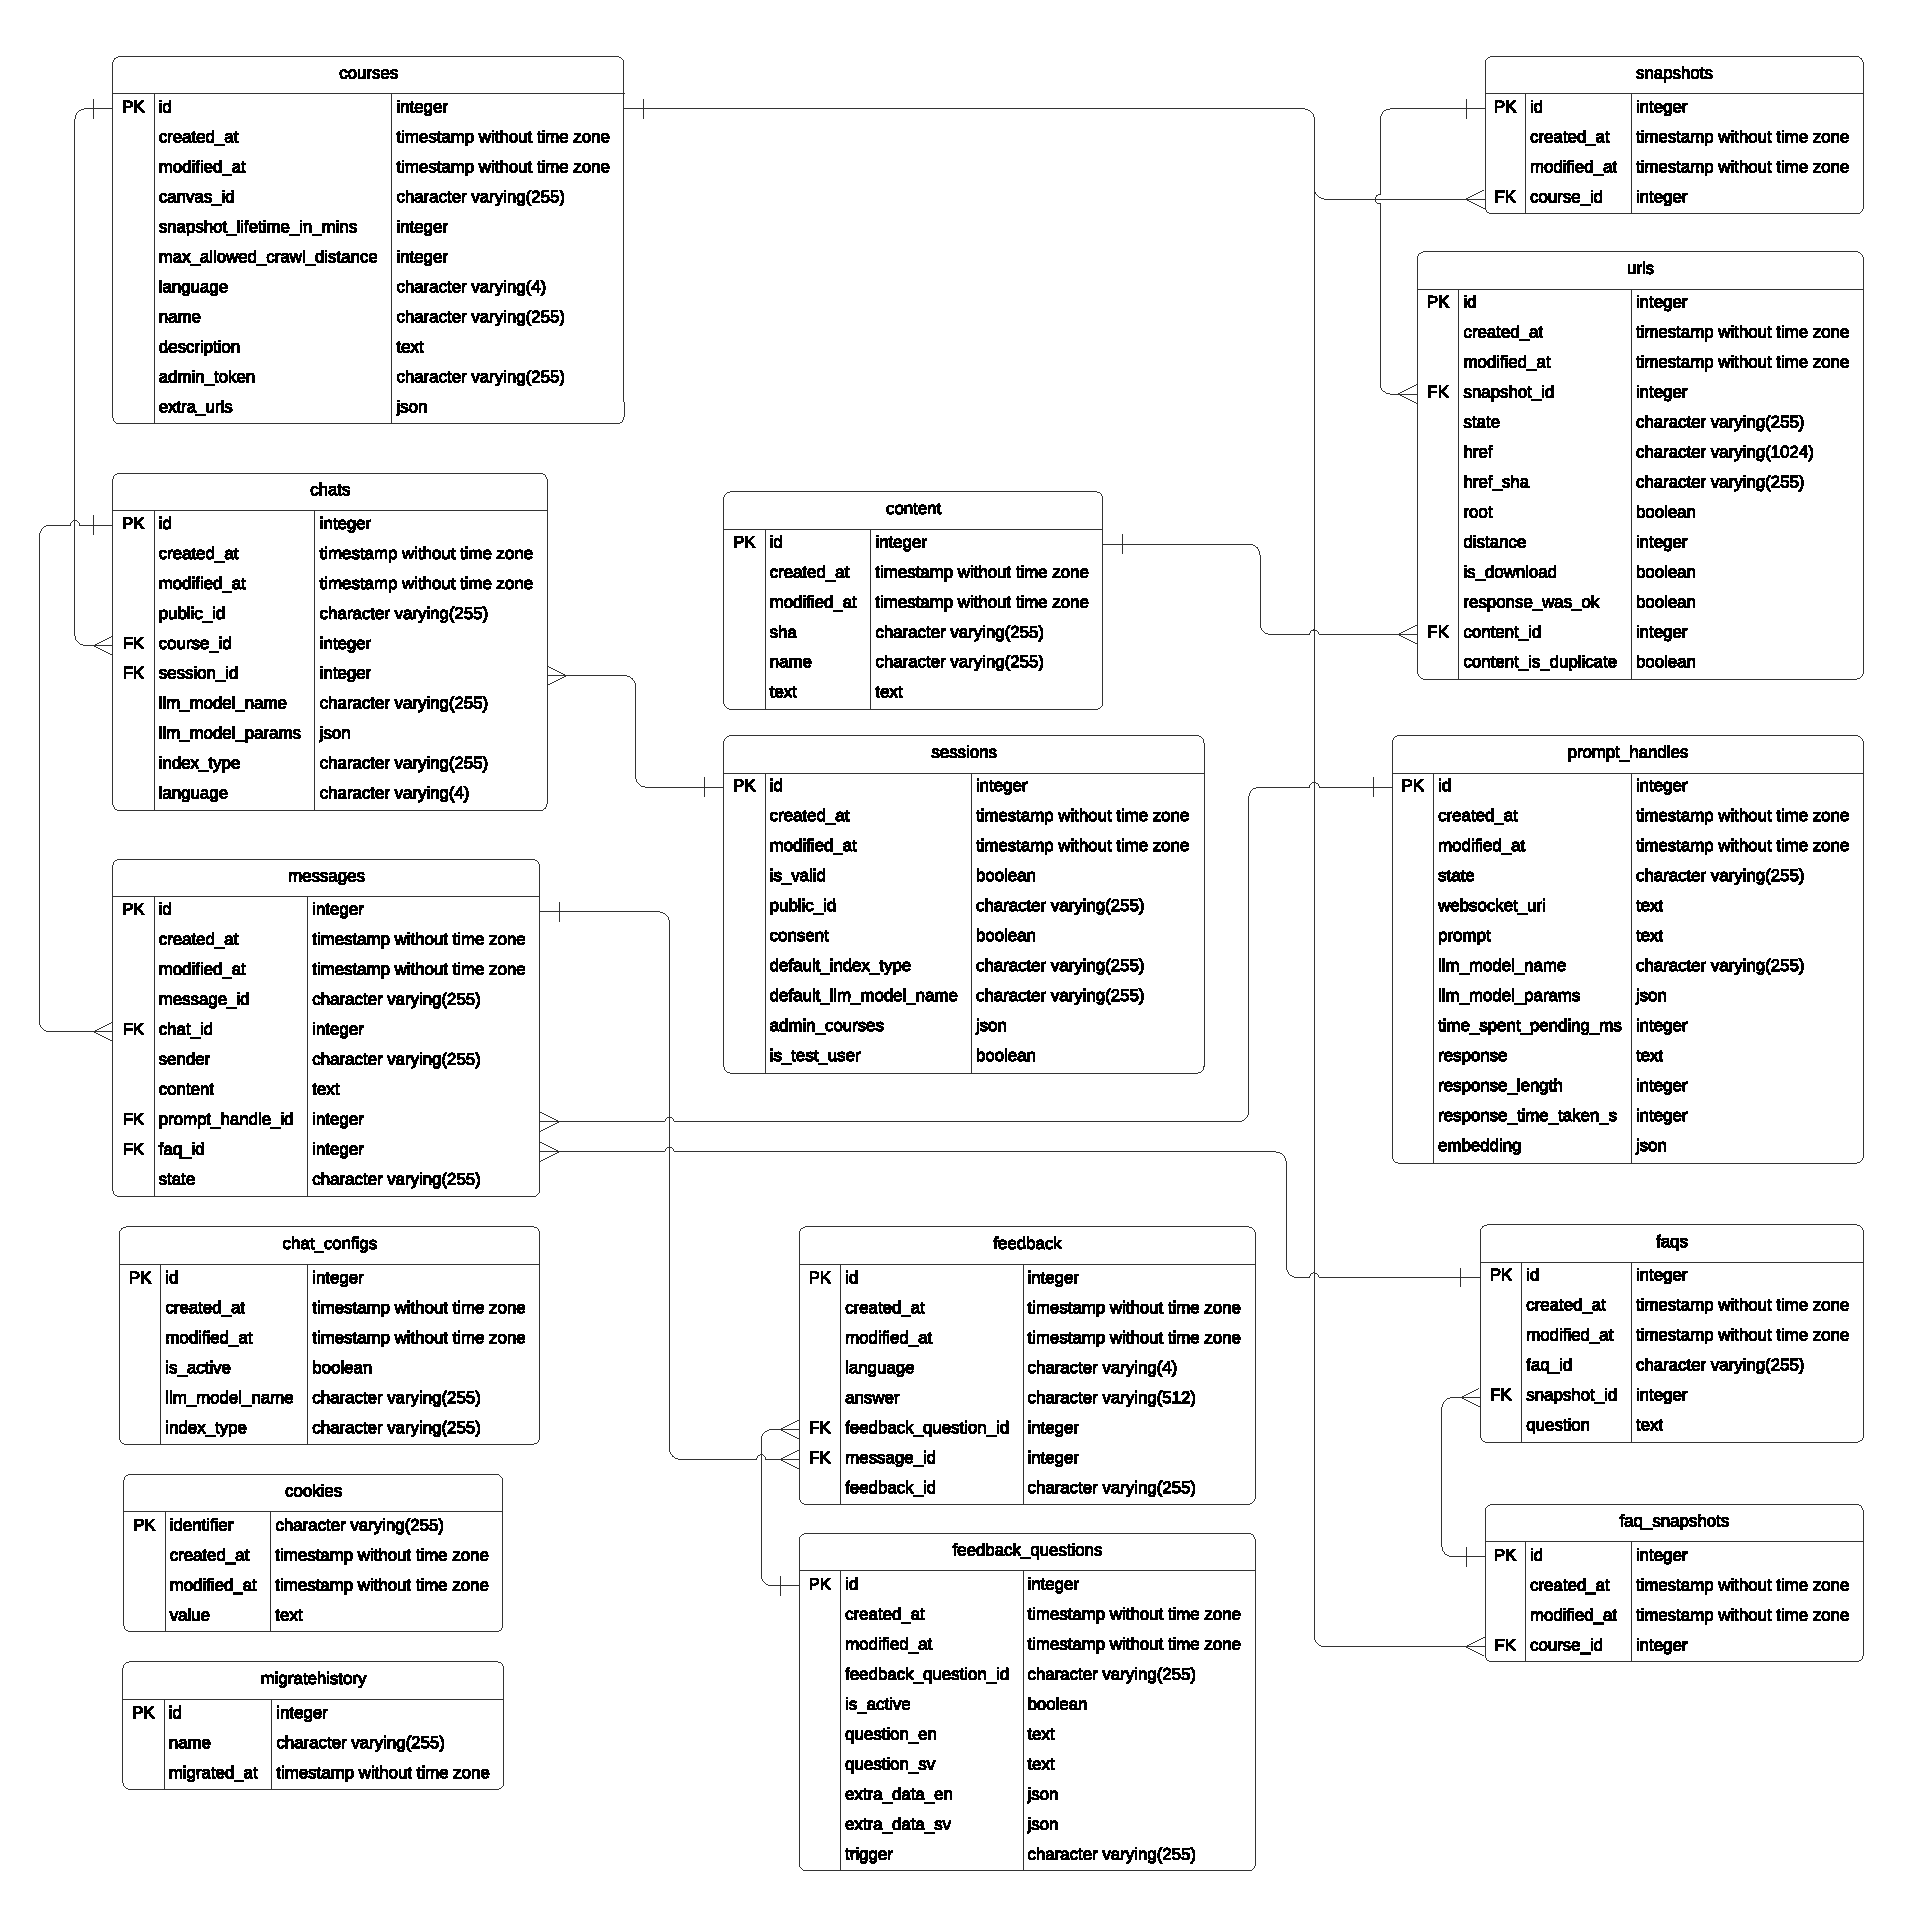
\includegraphics[width=\textwidth]{content/figures/assets/12-database-diagram.pdf}
    \caption{A diagram that shows the complete schema for the database}
    \label{fig:database_schema}
\end{figure}



\subsection{Document index}


Opensearch, which started as a fork of the popular search engine Elasticsearch, serves as a full text search backend and document store for the software. The opensearch server also stores each vector embedding for all supported vector embedding functions used in the study. Opensearch is also used in the software to compute similarity scores for the computed vector embeddings of all documents, utilising the k-NN algorithm for efficient nearest neighbour search. This enables rapid retrieval and ranking of relevant documents based on their vector similarities which is one of the key research goals of this thesis. Listing~\ref{fig:indexed_document} shows an example of a document indexed in a snapshot of a course room that participated in the study.


\begin{listing}[H]
\centering
\renewcommand{\theFancyVerbLine}{\scriptsize\arabic{FancyVerbLine}}
\scriptsize
\begin{minted}[
frame=lines,
framesep=2mm,
baselinestretch=1.2,
fontsize=\scriptsize,
linenos
]{json}
{
  "name": "Communication guidelines: DD1367 HT23 Programvarukonstruktion...",
  "text": "Document chunk: 1/1\nDocument summary: The document provides...",
  "text_raw": "Due to the mass amount of daily emails, I would like to...",
  "url": "https://canvas.kth.se/courses/43604/modules/items/765971",
  "sfr_embedding_mistral": [
    0.012644807808101177,
    -0.007494120392948389,
    0.005445912480354309,
    ...
  ],
  "text_embedding_3_large": [
    -0.009533963166177273,
    0.01081753708422184,
    -0.01858356036245823,
    ...
  ]
}
\end{minted}
\caption{Example of an indexed document from the course \textit{DD1367 Software Engineering in Project Form 9.0 credits} which participated in the study.}
\label{fig:indexed_document}
\end{listing}



\subsection{Running large language models at scale}


One of the principal requirements for the study software was the ability to investigate the impact of different \gls{LLM} on the experience of the user. This could impact the recall abilities of the system due to the models involvement in both understanding what the user is searching for and for summarising that information. Additionally, large embedding models would also be investigated within the scope of the study.


Proprietary models, such as those provided by OpenAI and are studied in this thesis, are always executed on the model vendors infrastructure and are accessible only via an HTTP API. These APIs are not compute-intensive for the consuming application, such as the one developed for this thesis. However, open-source models, like the Mistral family of models, are available for anyone to run. One of the goals of this thesis was to investigate the feasibility of running such applications with all necessary dependencies on-premise. This involved executing these models within the application. This presents an engineering challenge, as these models are not very mature yet, and the infrastructure for running them is not well developed.


For the software in this study an \textit{LLM-service} was developed. This service presented a high-level API that could be used by any part of the application, such as the chat-service, for producing messages, or the indexing service, for producing summaries or embeddings. The API had a high-level function that took a model name, model parameters and prompt to execute, and returned a prompt handle as a response. The data model for a prompt handle can be seen in its entirety in figure~\ref{fig:database_schema}, but in addition to the provided arguments, this kept the necessary queuing information for the system to function, some performance metrics and the output of the model.


In the background the service provides the infrastructure for organising a virtually unbounded number of worker-nodes for each model. Any worker node keeps the model running in memory, which could be either in CPU or GPU memory. Loading the model into memory is a time-consuming operation, which was one of the driving reasons for this approach. This architecture allows for scaling the service to keep up-with-higher demand for prompt-completions. Heavy load could be caused by for instance, many users using the system simultaneously, or indexing one or more course rooms simultaneously.


Organising systems like this have many difficulties, particularly regarding the distributed nature of this architecture and the compute intensiveness of model inference. For instance, since the execution time of a prompt can be upwards of a minute, the worker nodes need the ability to stream the response back to an end user in real-time token-by-token, to provide a good user experience. For this reason a websocket service was implemented, that allows the end-user application to listen for tokens being produced over a websocket that the producing node is directly connected to. More advanced queue techniques, such as a Kafka queue, could have been implemented instead of using a database table with distributed mutex locks in Redis. However, for rapid implementation and prototyping, the chosen approach was adequate for the software in this thesis.
\subsection{Assigning a chat configuration to a user}


The system supports defining multiple chat configurations, each consisting of a specific set of tools and models for the user’s chat experience. A chat configuration consists of;


\begin{itemize}
        \item \textbf{A Language Model}: This is the \gls{LLM} used for generating assistant responses and computing internal agent functionality such as the post processing of documents, if that’s enabled for the config.
        \item \textbf{Retrieval Technique}: The method used for information retrieval, either an embedding model or full-text search.
        \item \textbf{Embedding Model}: Specifies the embedding model if used.
        \item \textbf{Document Processing}: Indicates whether documents should be post-processed before being inserted into the chat context (see section~\ref{sec:post_processing}).
\end{itemize}


Any configuration can be selectively enabled or disabled based on the experimental requirements.

When a user accesses the system for the first time, a configuration is randomly assigned to ensure an unbiased distribution among users. Once assigned, the configuration remains consistent for the lifetime of that user’s account. This is however only true if the user uses the same browser, a new browser would result in a separate account.


\subsection{Gathering user feedback}
\label{sec:what_you_did_gathering_feedback_data}


The software was designed to facilitate user feedback collection. This feedback is gathered through a fairly flexible feedback entity, which integrates questions in the configured language of the course. A feedback questions are triggered by specific conditions, such as:


\begin{itemize}
\item After the response for the $n$-th message is sent in the $m$-th chat a user has had, where $n$ represent the number of messages in the current chat and $m$ the number of chat a user have had in total.
\item After generating a response to a frequently asked question.
\end{itemize}


These triggers were chosen to capture the user experience over a certain period, enabling control over the duration of system usage when analysing the users response to each feedback question.


The feedback question format was designed to be extensive. There were two formats implemented for the research in this thesis. These formats were multiple choice questions, and binary \textit{thumbs up} / \textit{thumbs down} questions. Figure~\ref{fig:multiple_choice}~and~\ref{fig:feedback_thumbs} showcase these two formats respectively.


\begin{figure}[H]
    \centering
    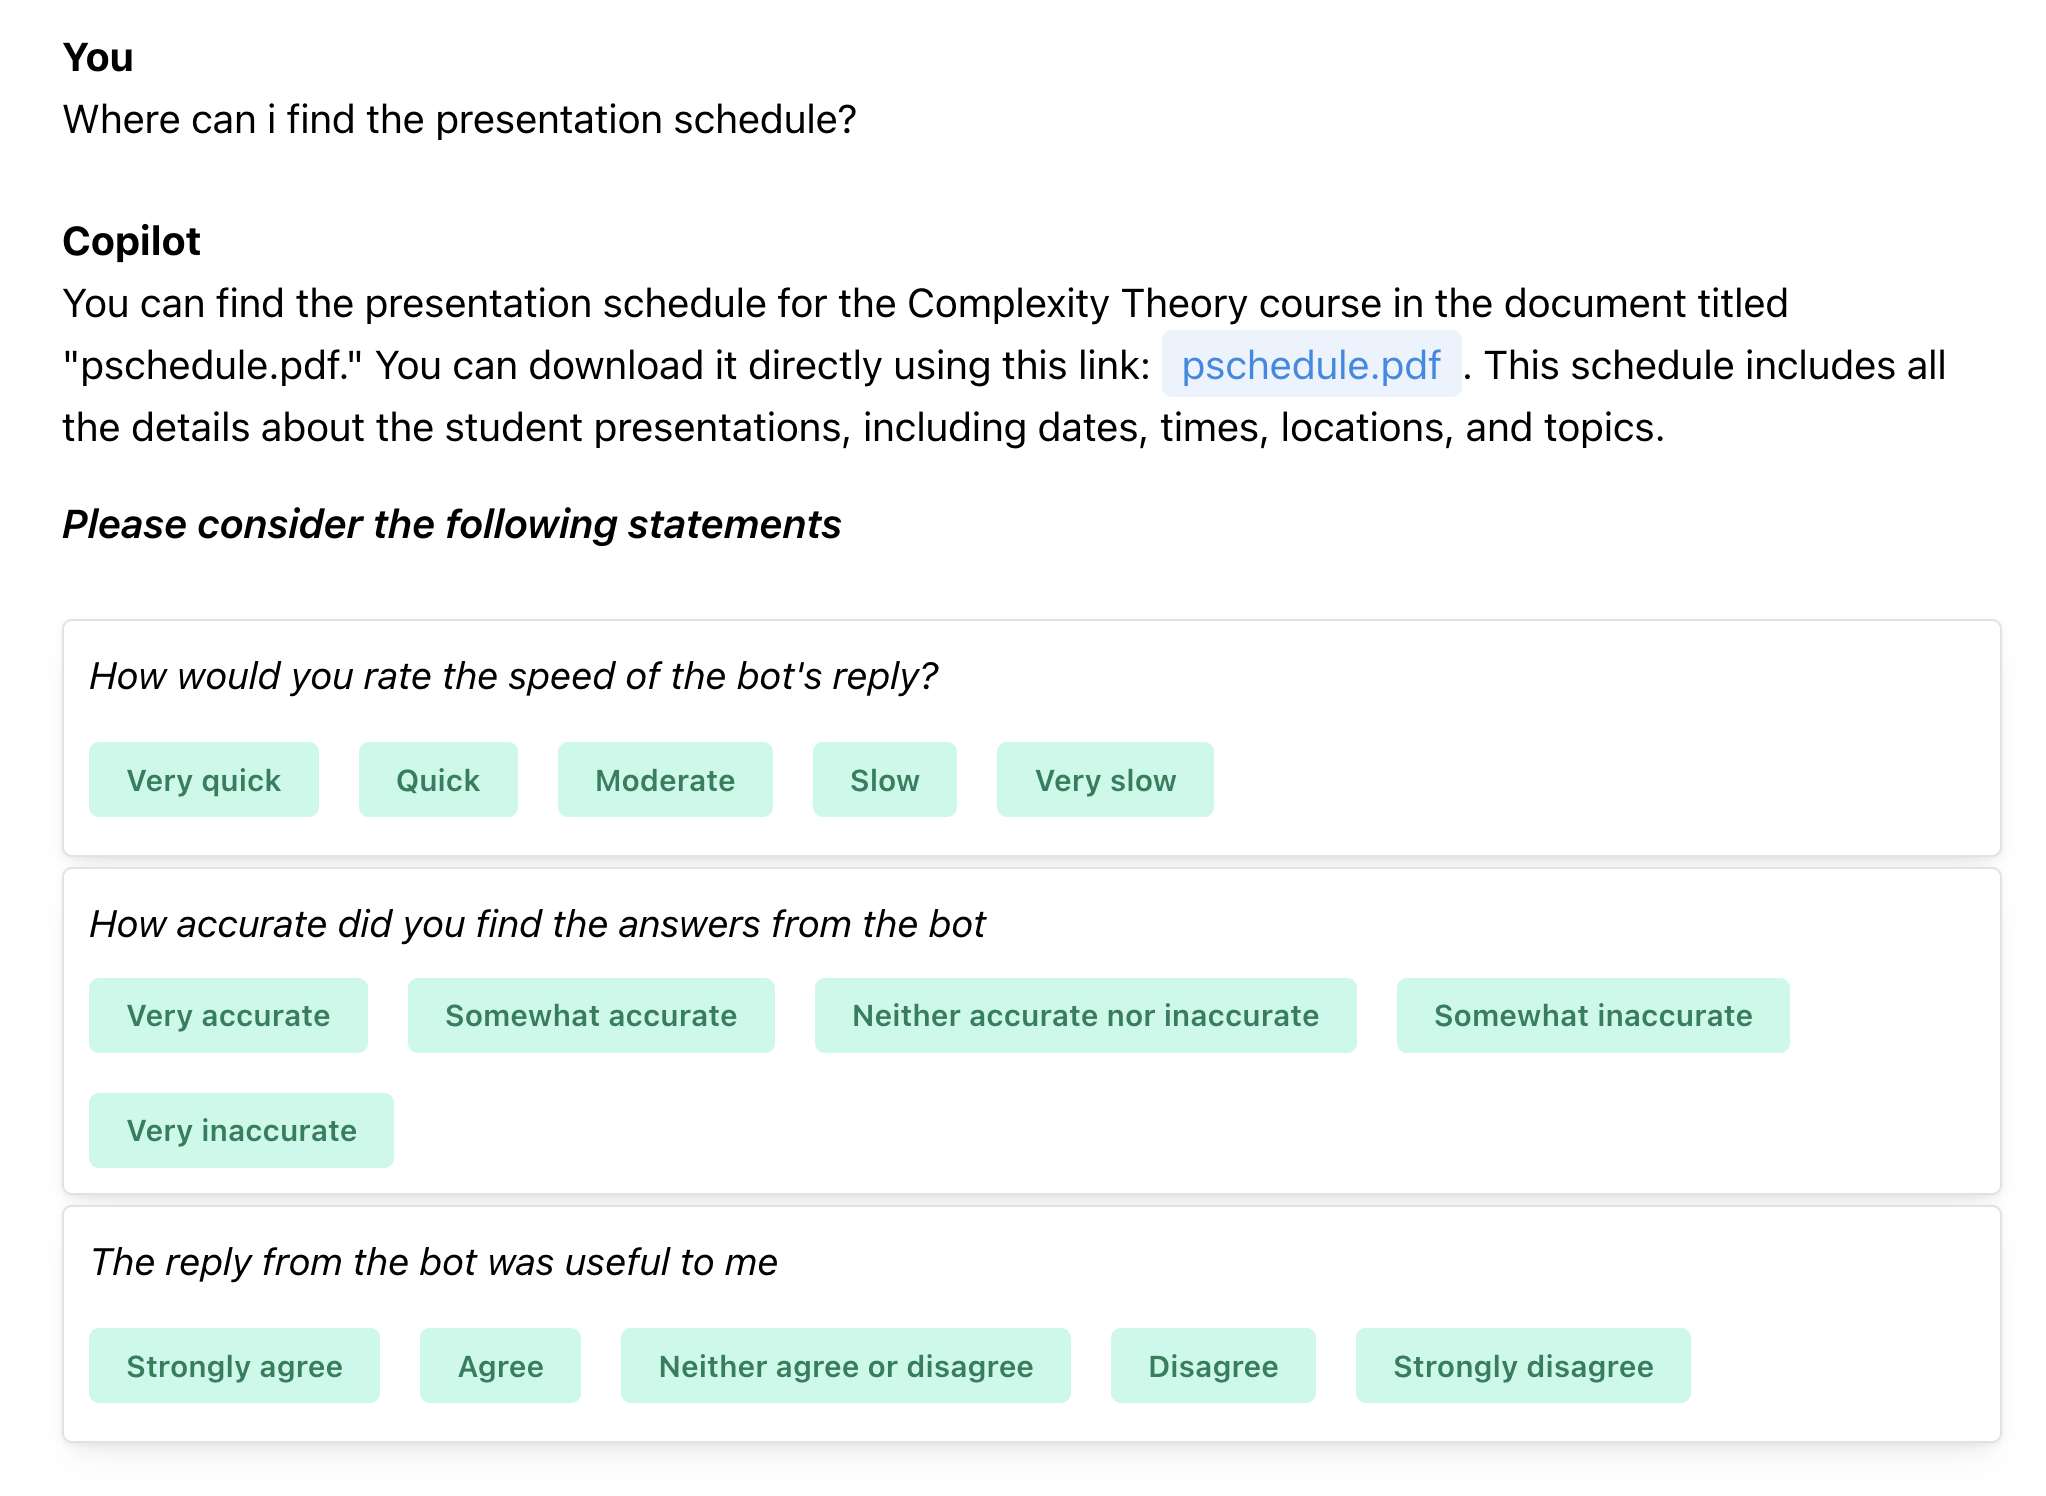
\includegraphics[width=\textwidth]{content/figures/assets/15-feedback-choices.png}
    \caption{Example of a number of multiple choice questions inserted into the chat}
    \label{fig:multiple_choice}
\end{figure}



\begin{figure}[H]
    \centering
    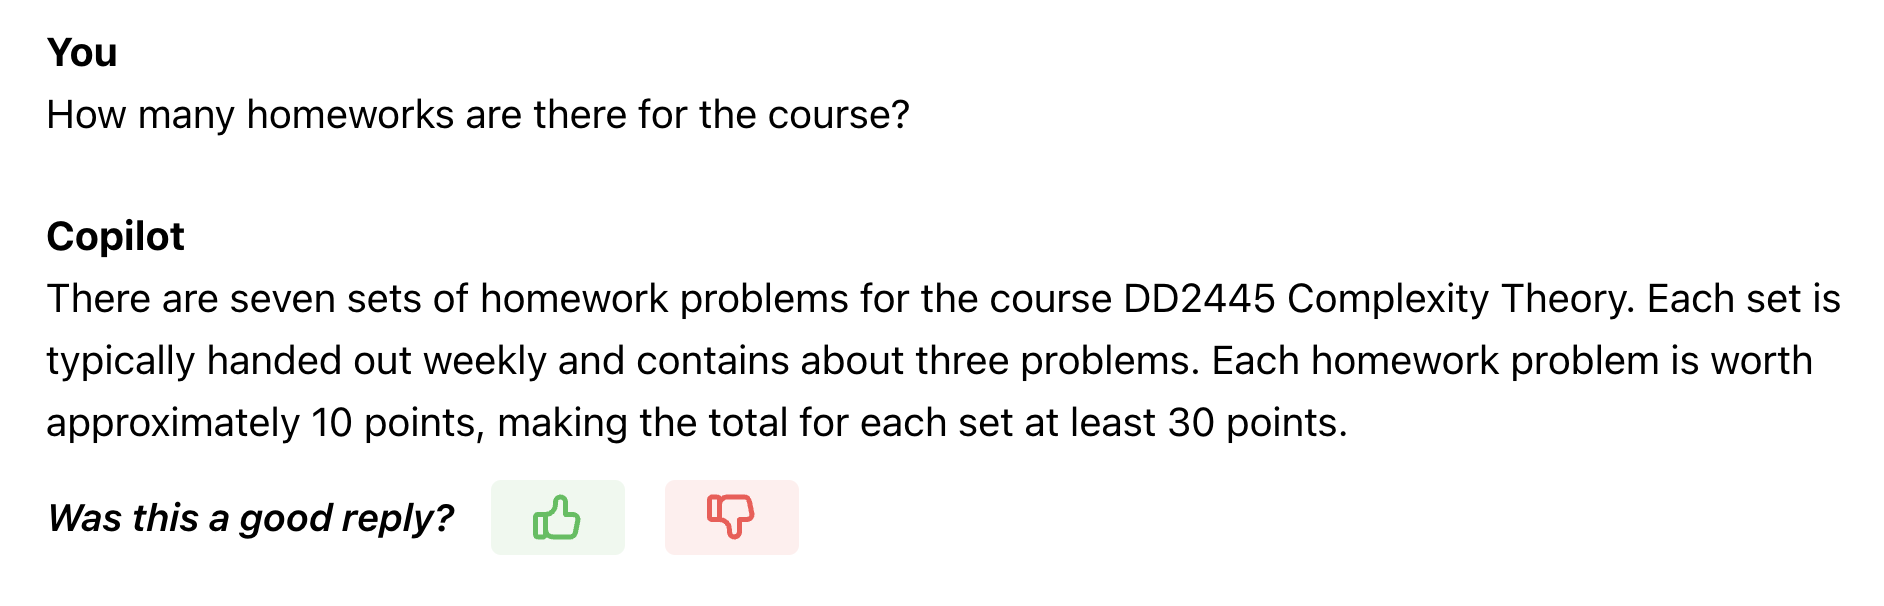
\includegraphics[width=\textwidth]{content/figures/assets/14-feedback-thumbs.png}
    \caption{Example of a thumbs up/thumbs down question inserted into the chat after the user clicks on a FAQ.}
    \label{fig:feedback_thumbs}
\end{figure}



\subsection{User interface}


The assistant built for the system was designed to live within the \gls{LMS} used at KTH, known as canvas. Each couse in canvas is assigned a course room. This course room contains all the information a participant in the course might need, such as course announcement, assignments and modules. \autoref{fig:canvas_course_room} shows the course room of one of the courses that participated in the study. The \gls{GUI} for the assistant designed for this thesis, was designed to live within the courseroom as an iframe.


The software constructed for this study was designed to integrate with KTH's \gls{LMS}, Canvas. Each course in Canvas has a designated course room that contains all information for students in the course. This includes announcements, assignments, modules and more. \autoref{fig:canvas_course_room} shows the course room of one of the participating courses in the study. The \gls{GUI} for the assistant, developed for this thesis, was embedded within the course room as an iframe, accessible through the course sidebar in the web, and navigation menu in the Canvas mobile app.


\begin{figure}[H]
    \centering
    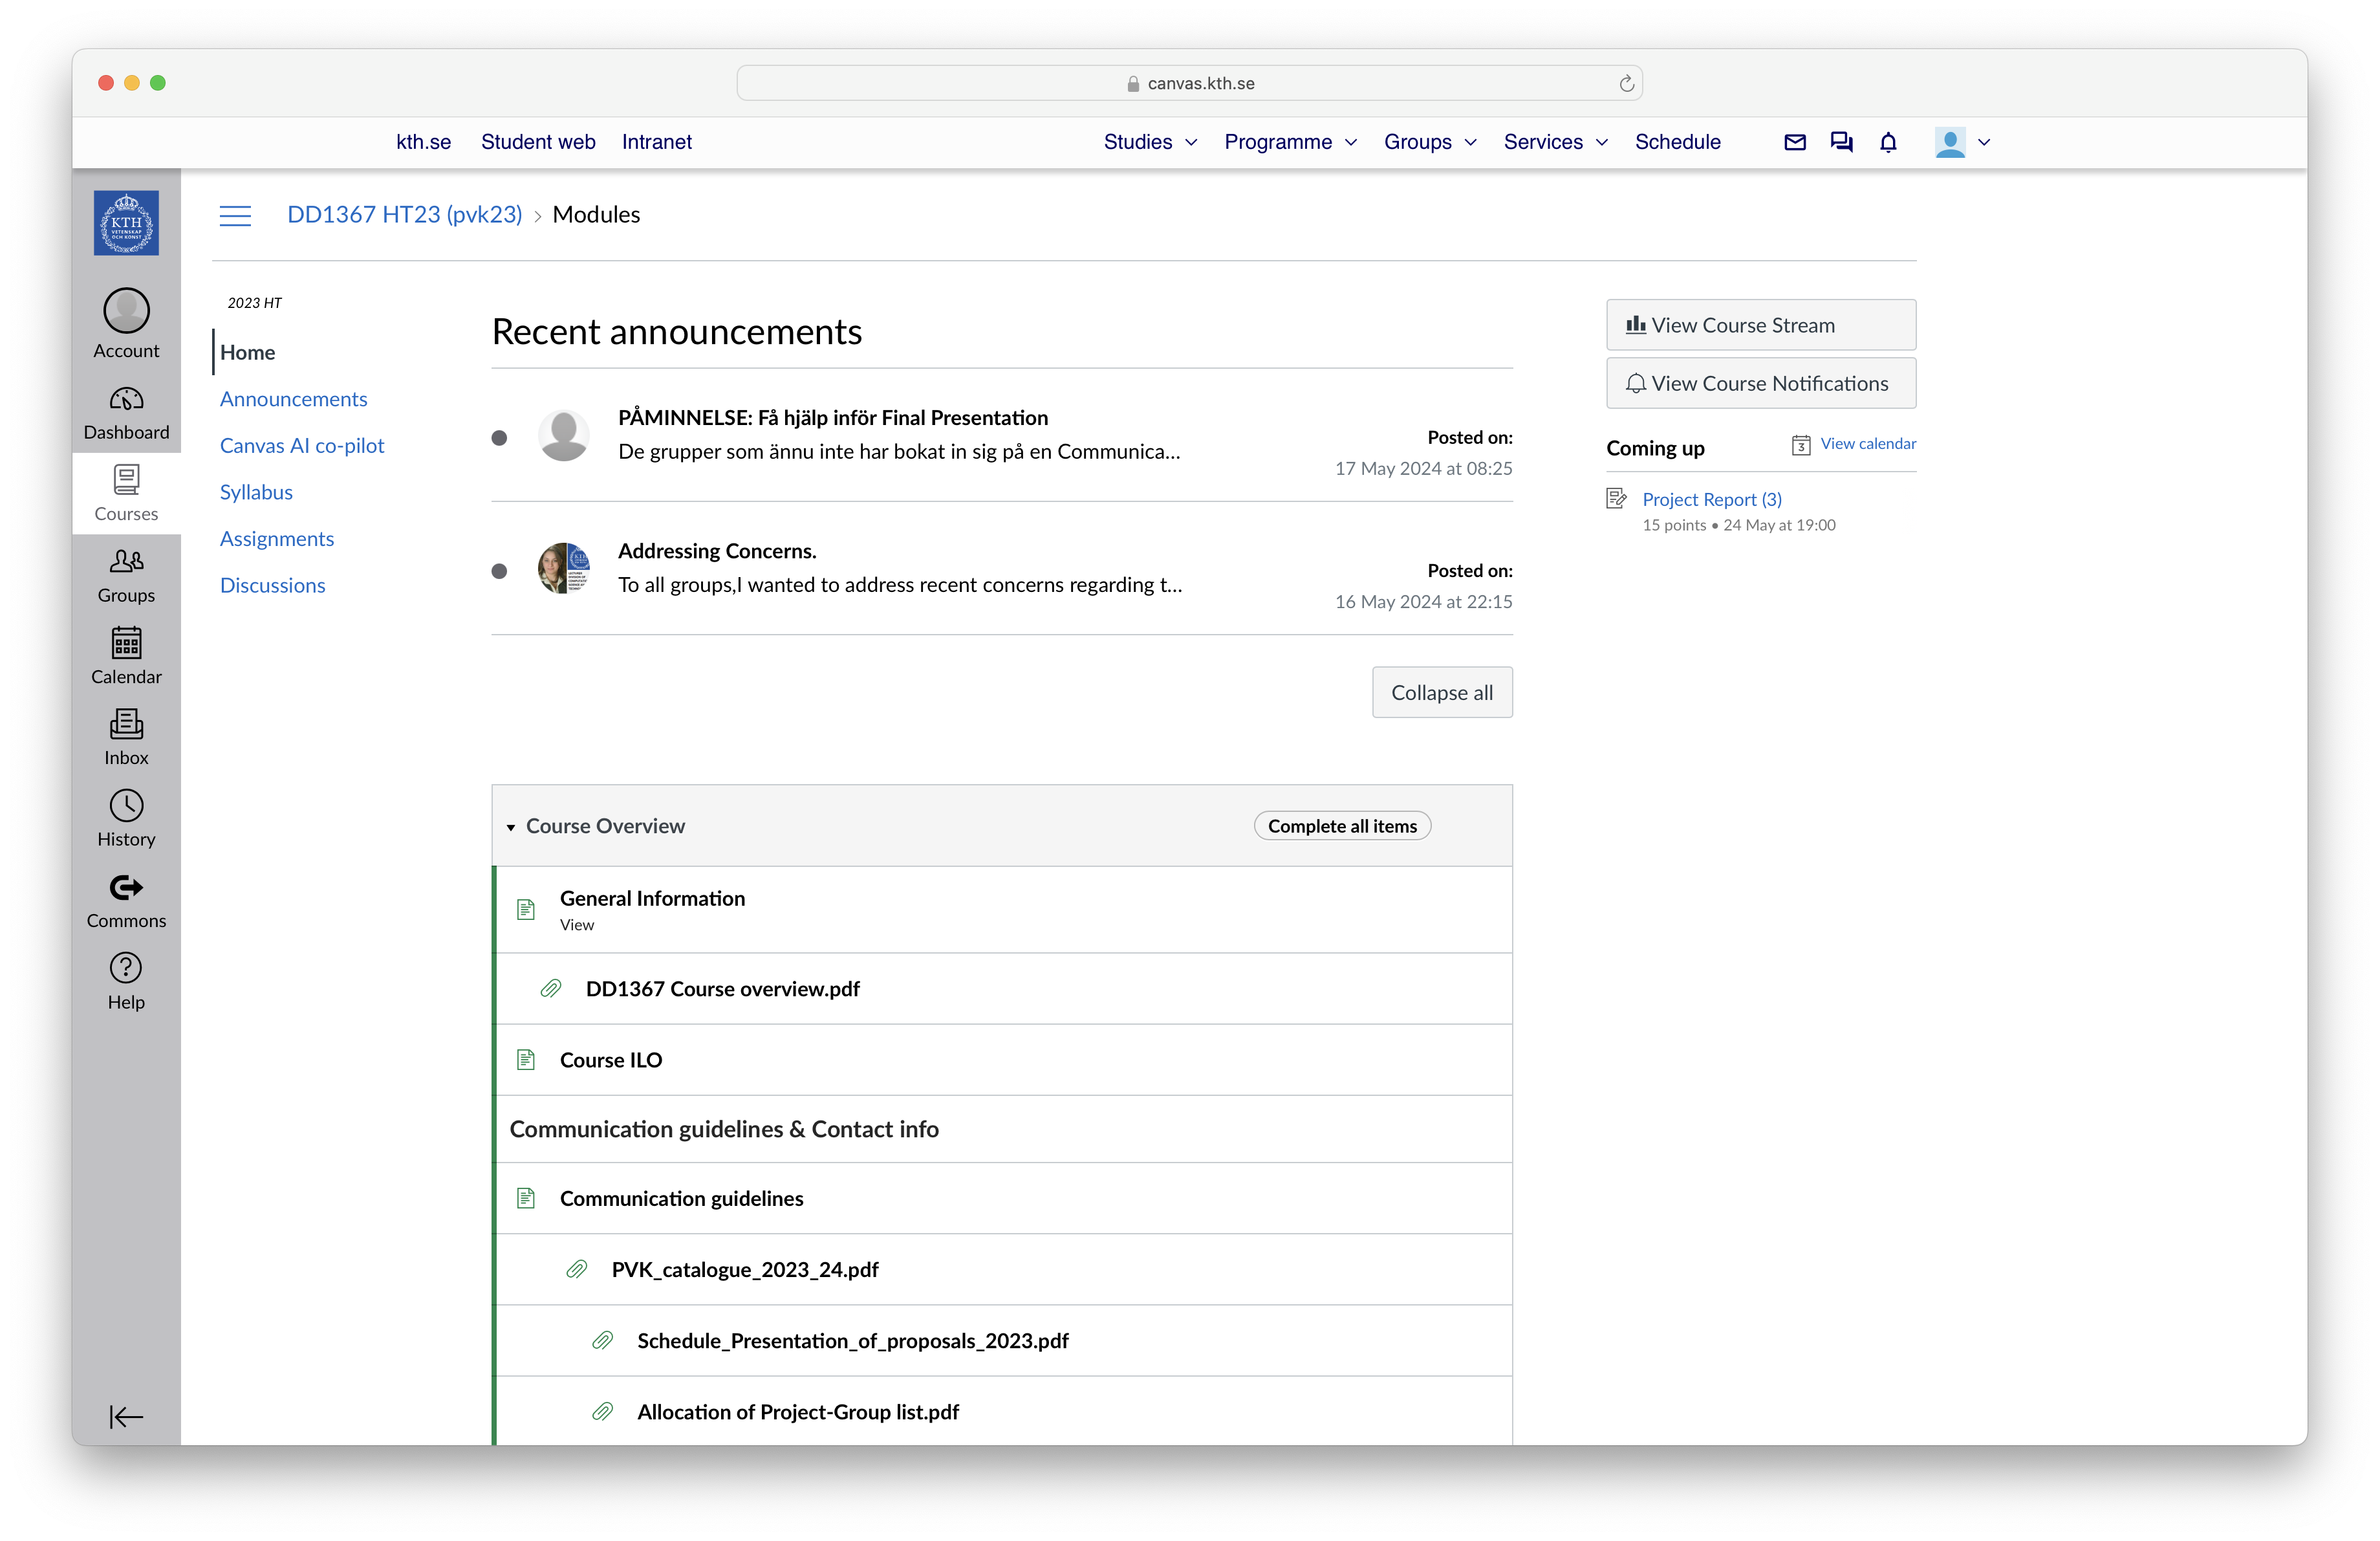
\includegraphics[width=\textwidth]{content/figures/assets/16-canvas-course-room.png}
    \caption{The course room of DD1367 Software Engineering in Project Form 9.0 credits in canvas}
    \label{fig:canvas_course_room}
\end{figure}



% \begin{figure}[H]
    \centering
    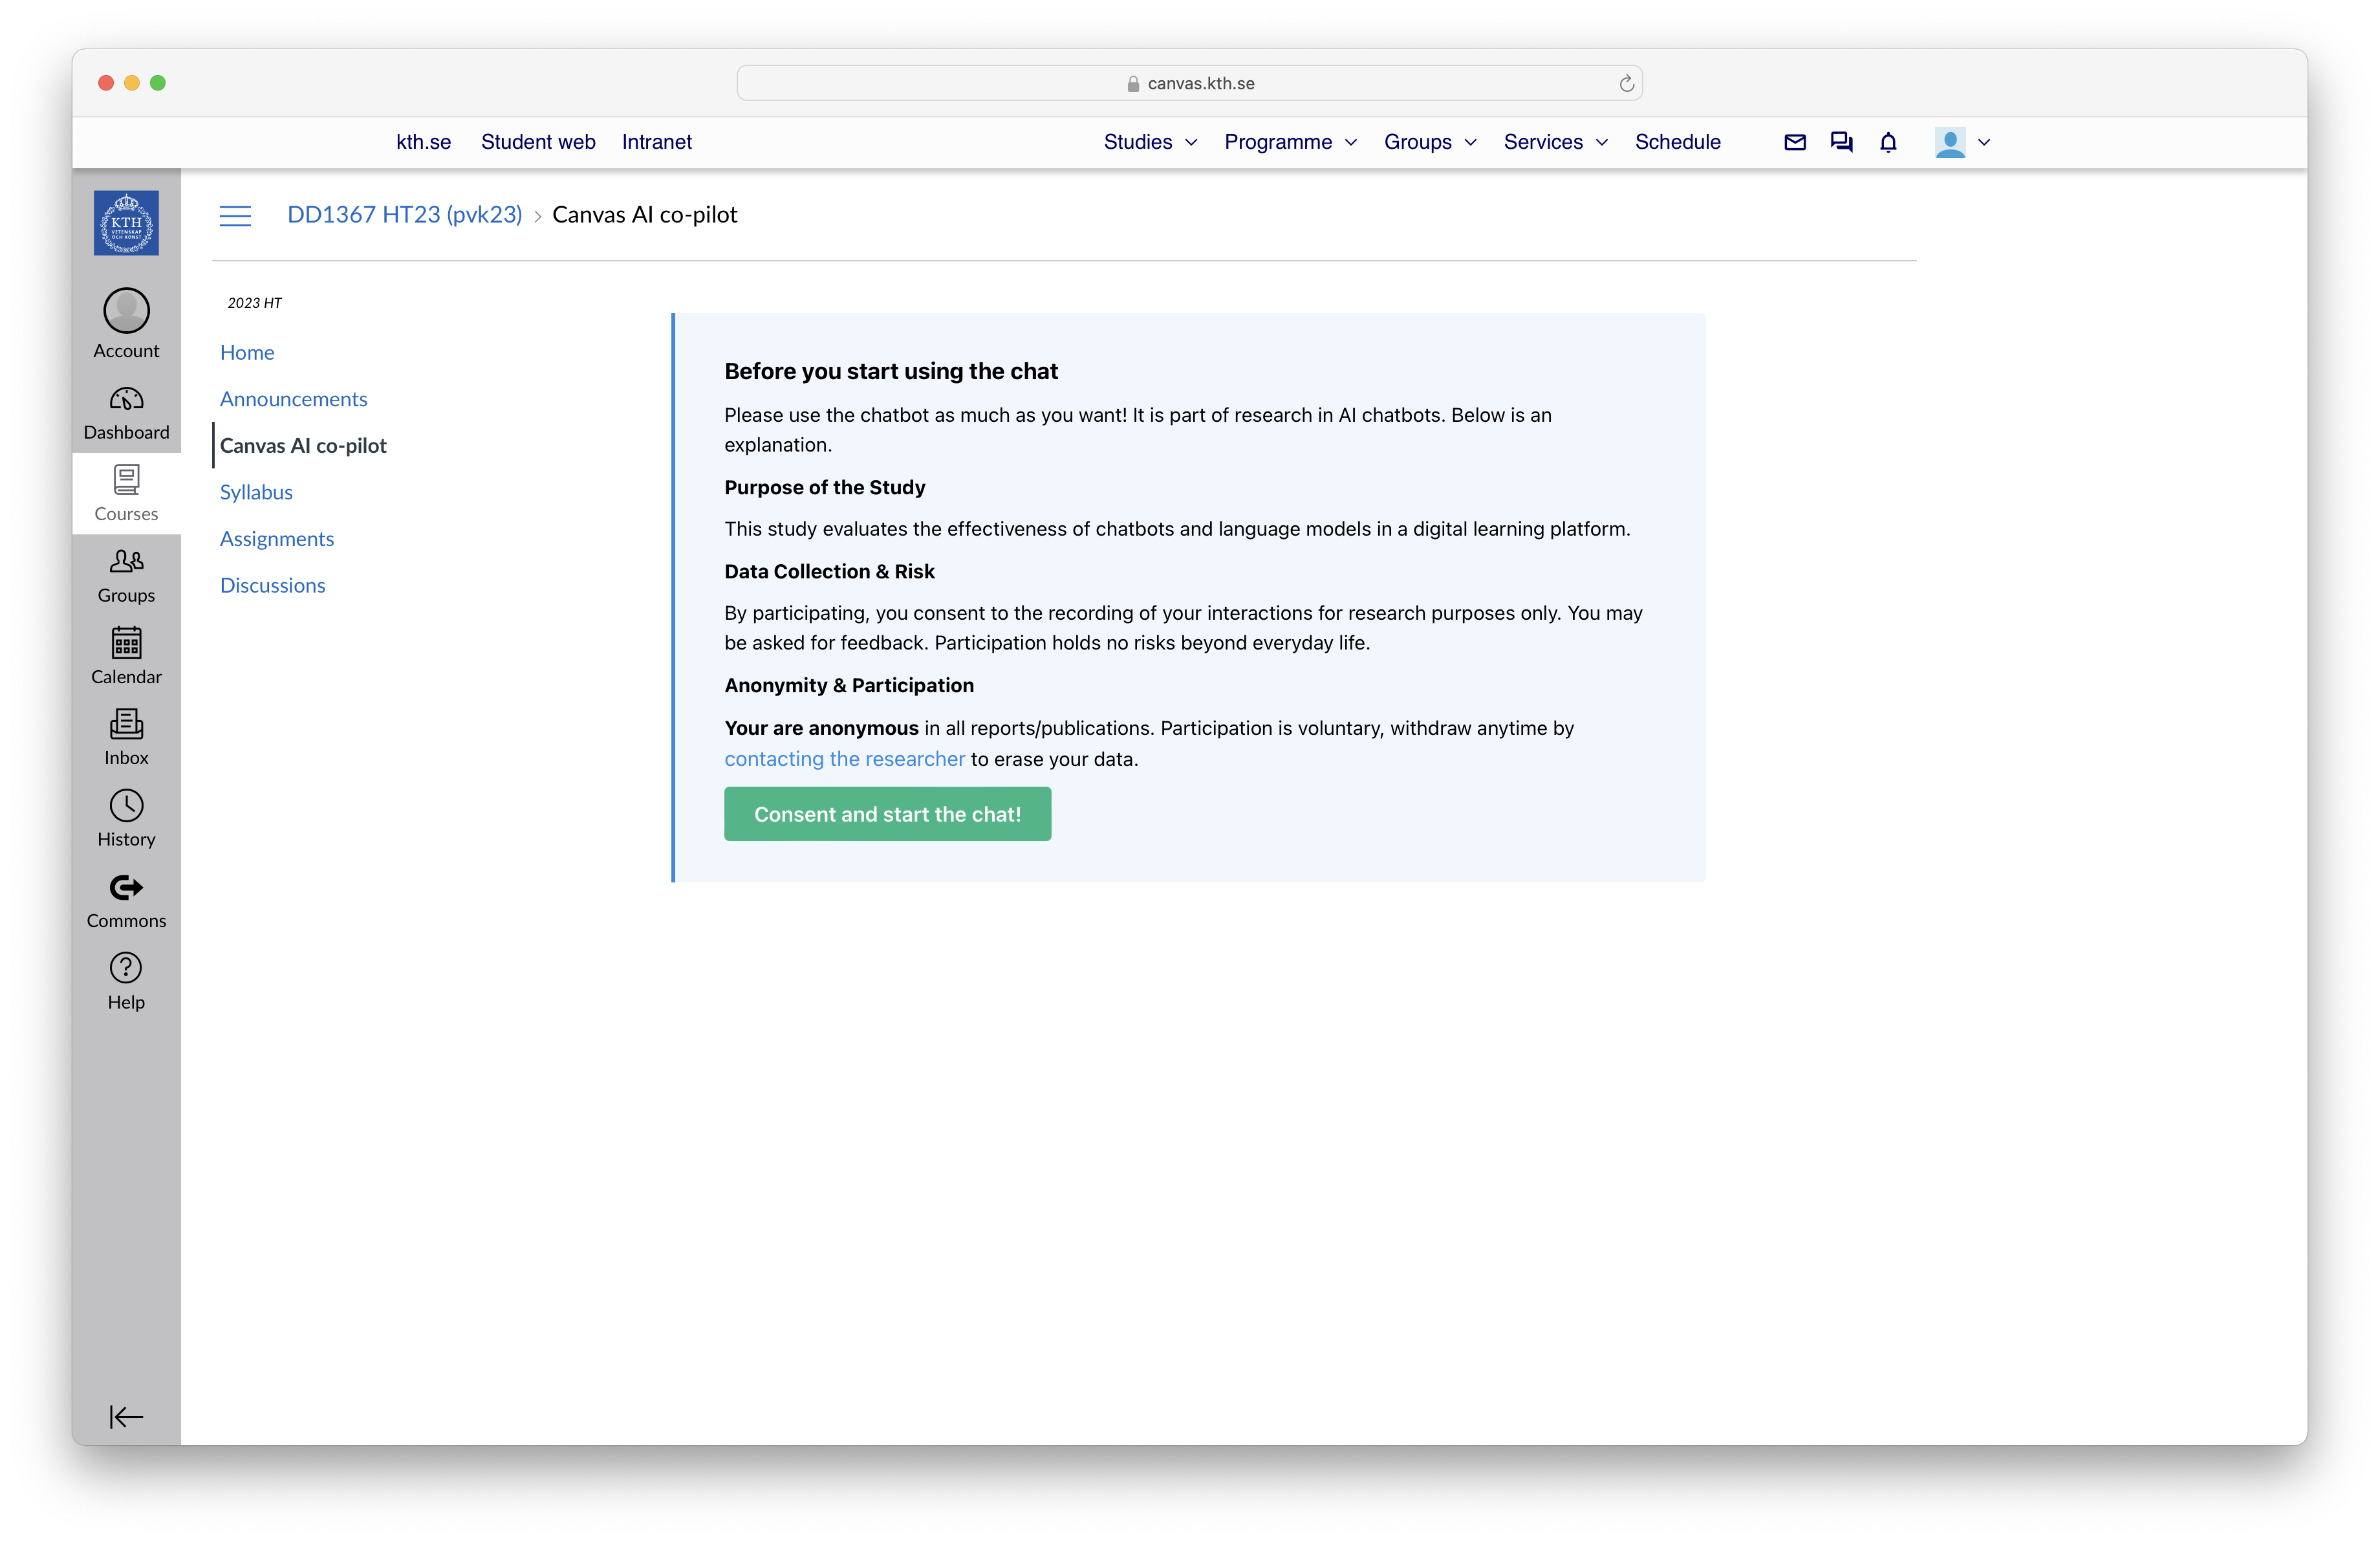
\includegraphics[width=\textwidth]{content/figures/assets/17-consent-form.png}
    \caption{The consent form shown to participants in the study before using the software}
    \label{fig:consent_form}
\end{figure}



The system utilise a script that compiles the most common questions. These are displayed each time a user starts the application, as can be seen in figure~\ref{fig:faq_questions}. This allows the user to quickly understand what other students have asked the tool, and quickly start a conversation.


\begin{figure}[H]
    \centering
    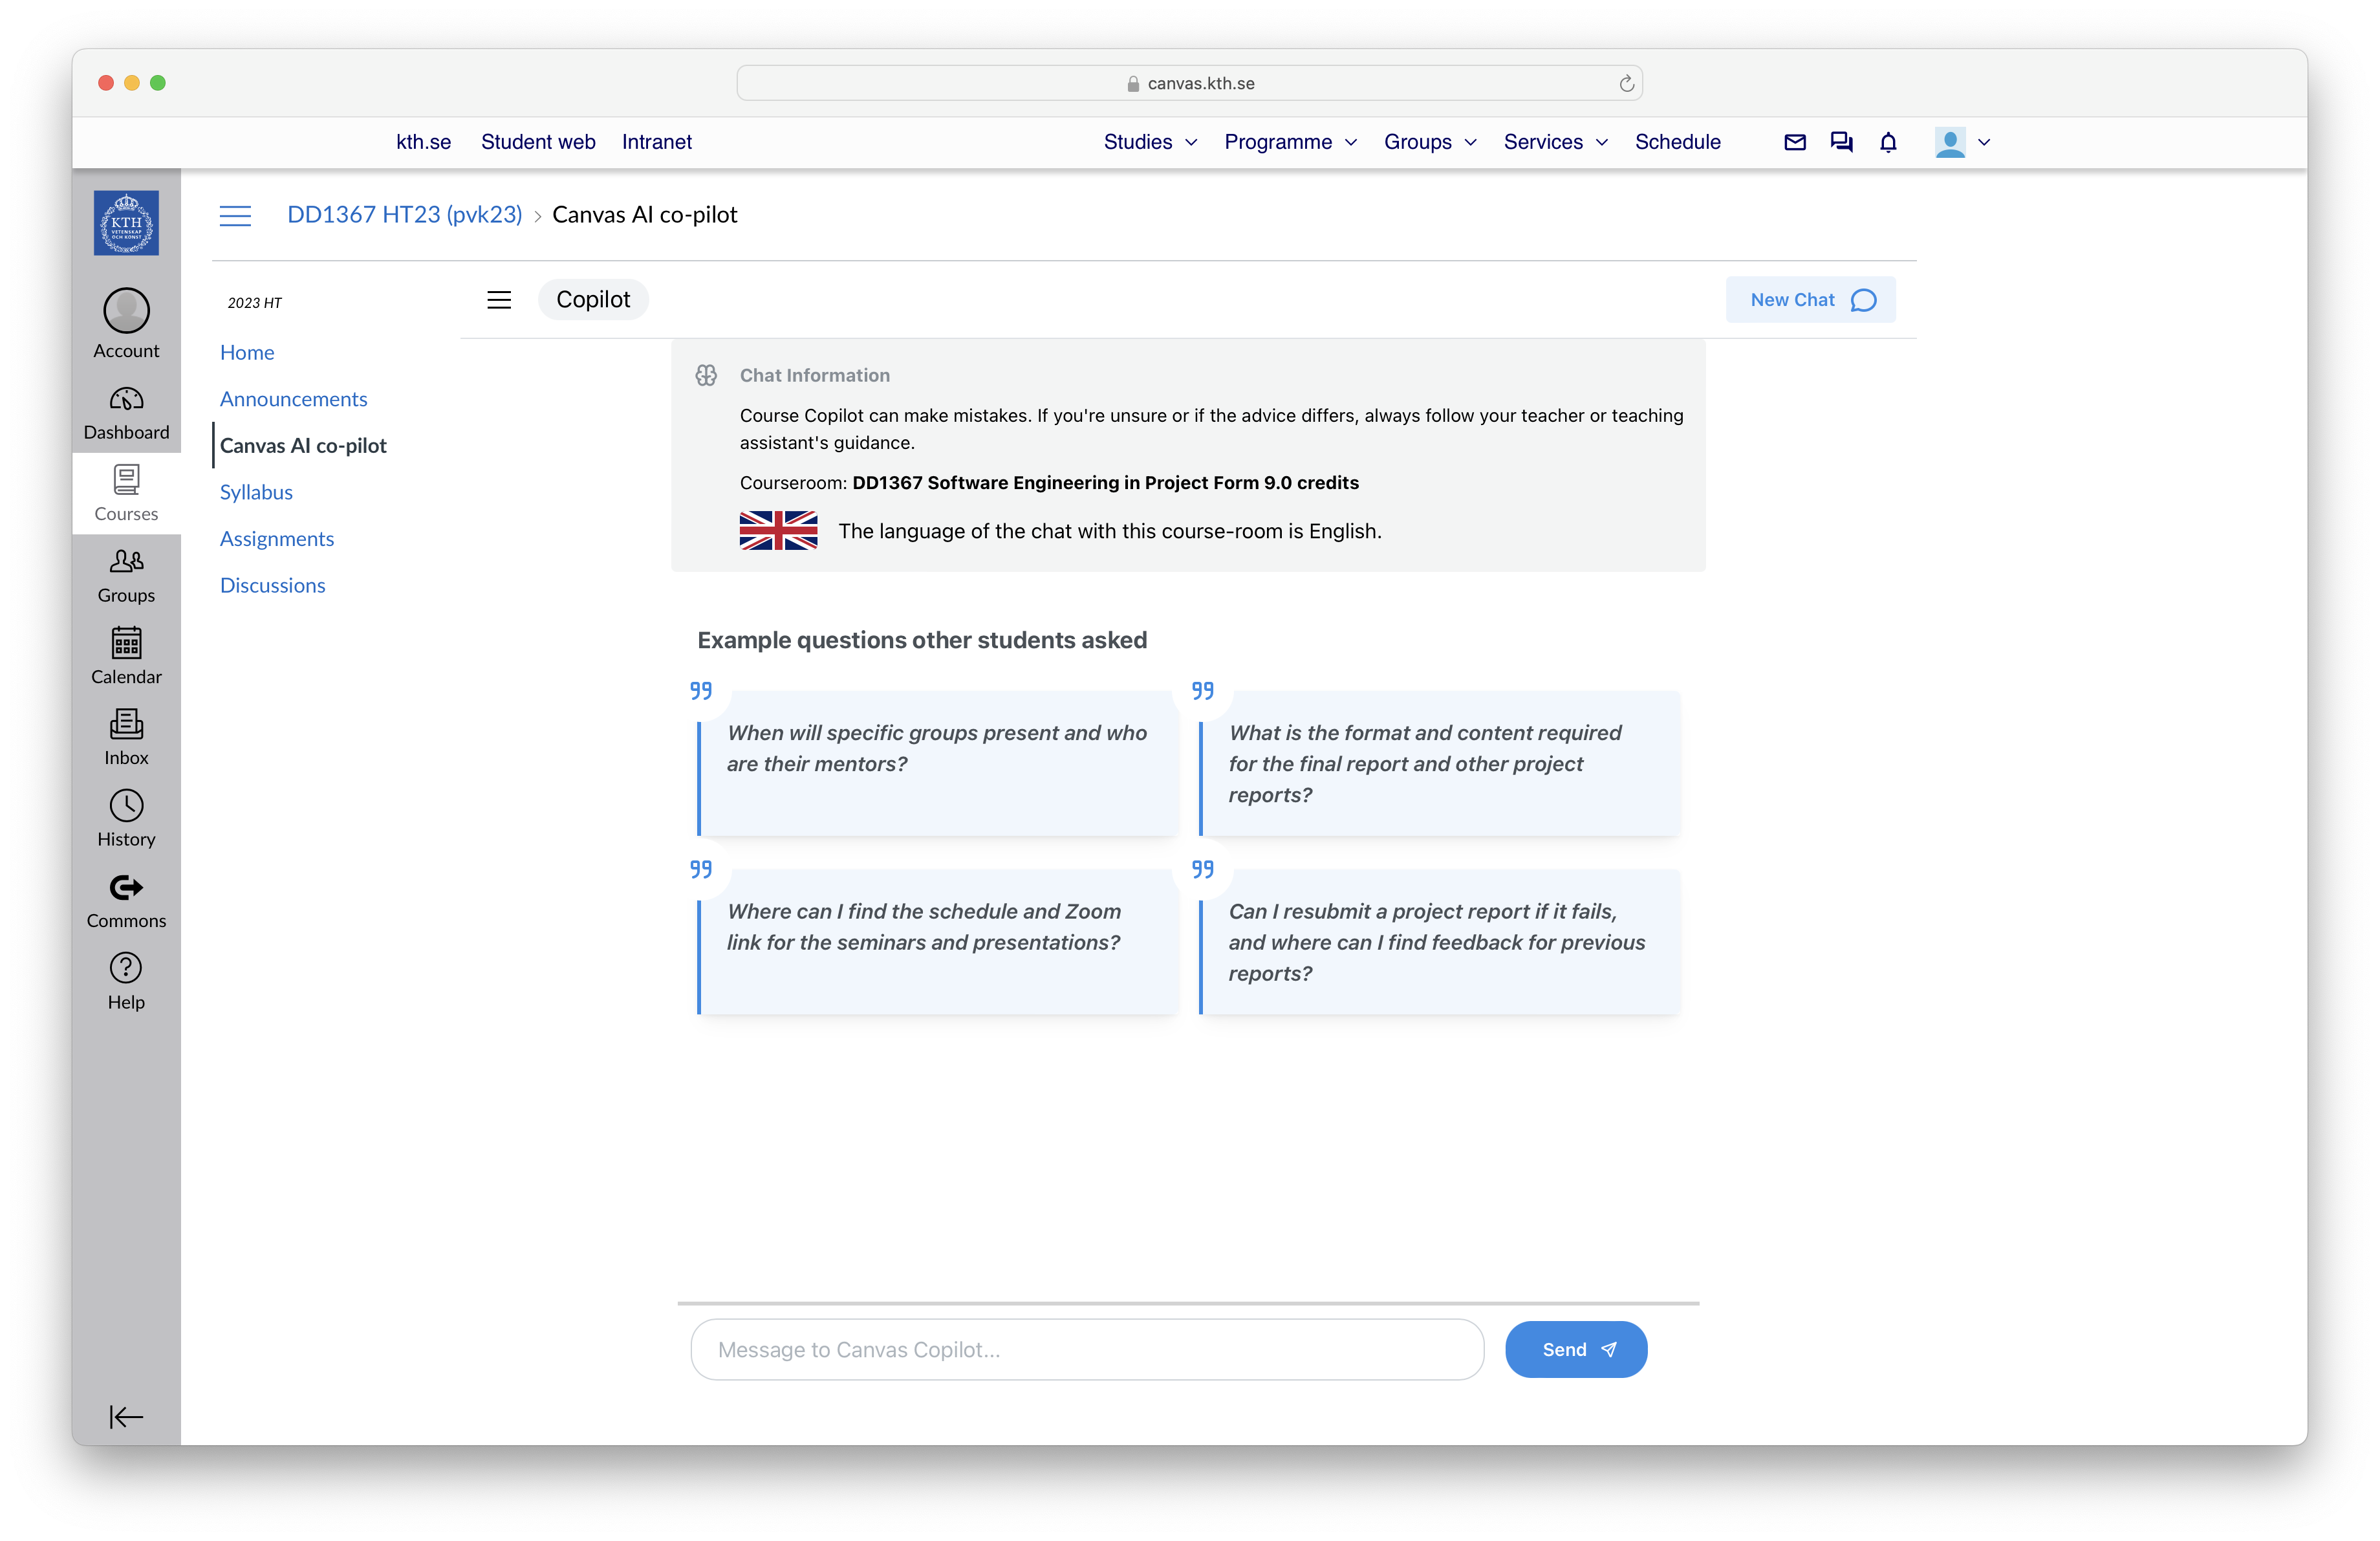
\includegraphics[width=\textwidth]{content/figures/assets/18-faq-questions.png}
    \caption{The chat UI with frequently asked questions shown before the user sends their first message}
    \label{fig:faq_questions}
\end{figure}



Overall, the \gls{GUI} of the tool is very simple as can be seen in figure~\ref{fig:conversation_with_assistant}. It allows users to send and receive messages from the tool. The responses from the assistant support some rich formatting, such as bold fonts. Links to cited documents are highlighted and forwards the user to the corresponding page or file in canvas when clicked. A video demonstration of the software being used by a student \href{https://www.youtube.com/watch?v=spdZ4jwI8mo}{can be seen here}.


Any teacher or TA can be granted administrative privileges which yields them access to a list of all chats that have been had between students and the assistant in their course. This allows them insights into what the chatbot is responding to the students' questions.


\begin{figure}[H]
    \centering
    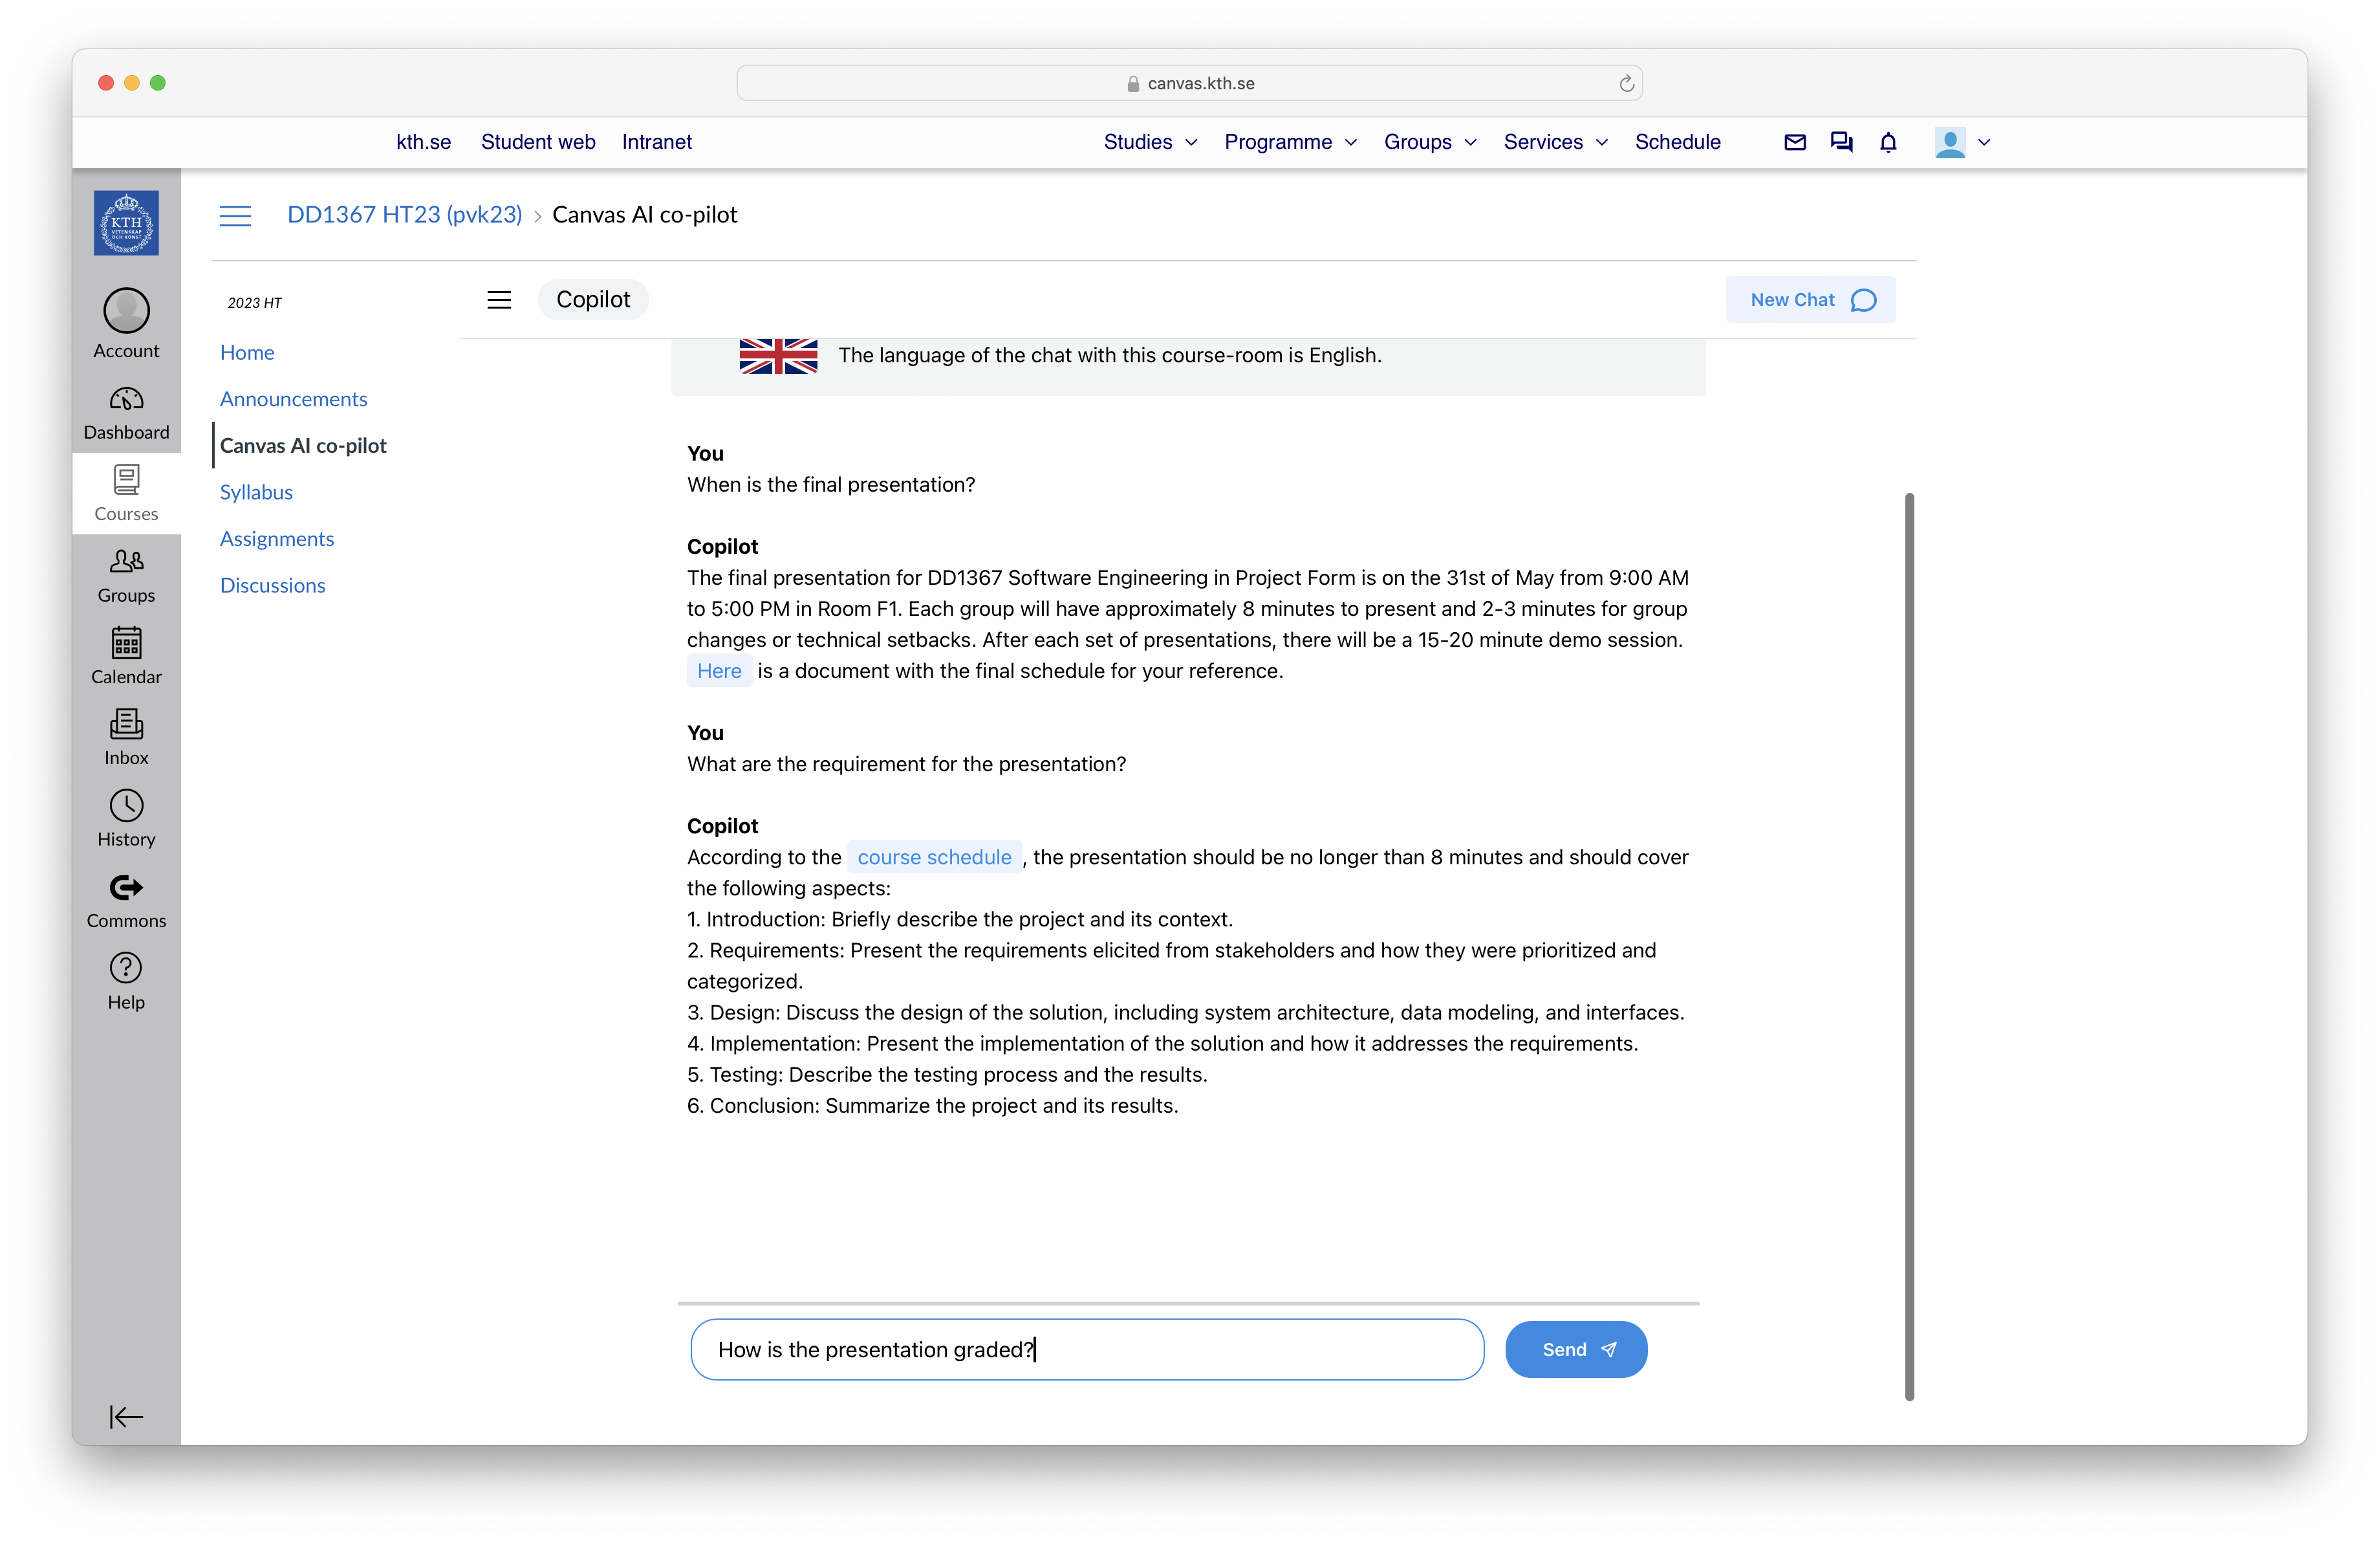
\includegraphics[width=\textwidth]{content/figures/assets/19-a-conversation-with-the-assistant.png}
    \caption{A short conversation with the assistant}
    \label{fig:conversation_with_assistant}
\end{figure}



% \begin{figure}[H]
    \centering
    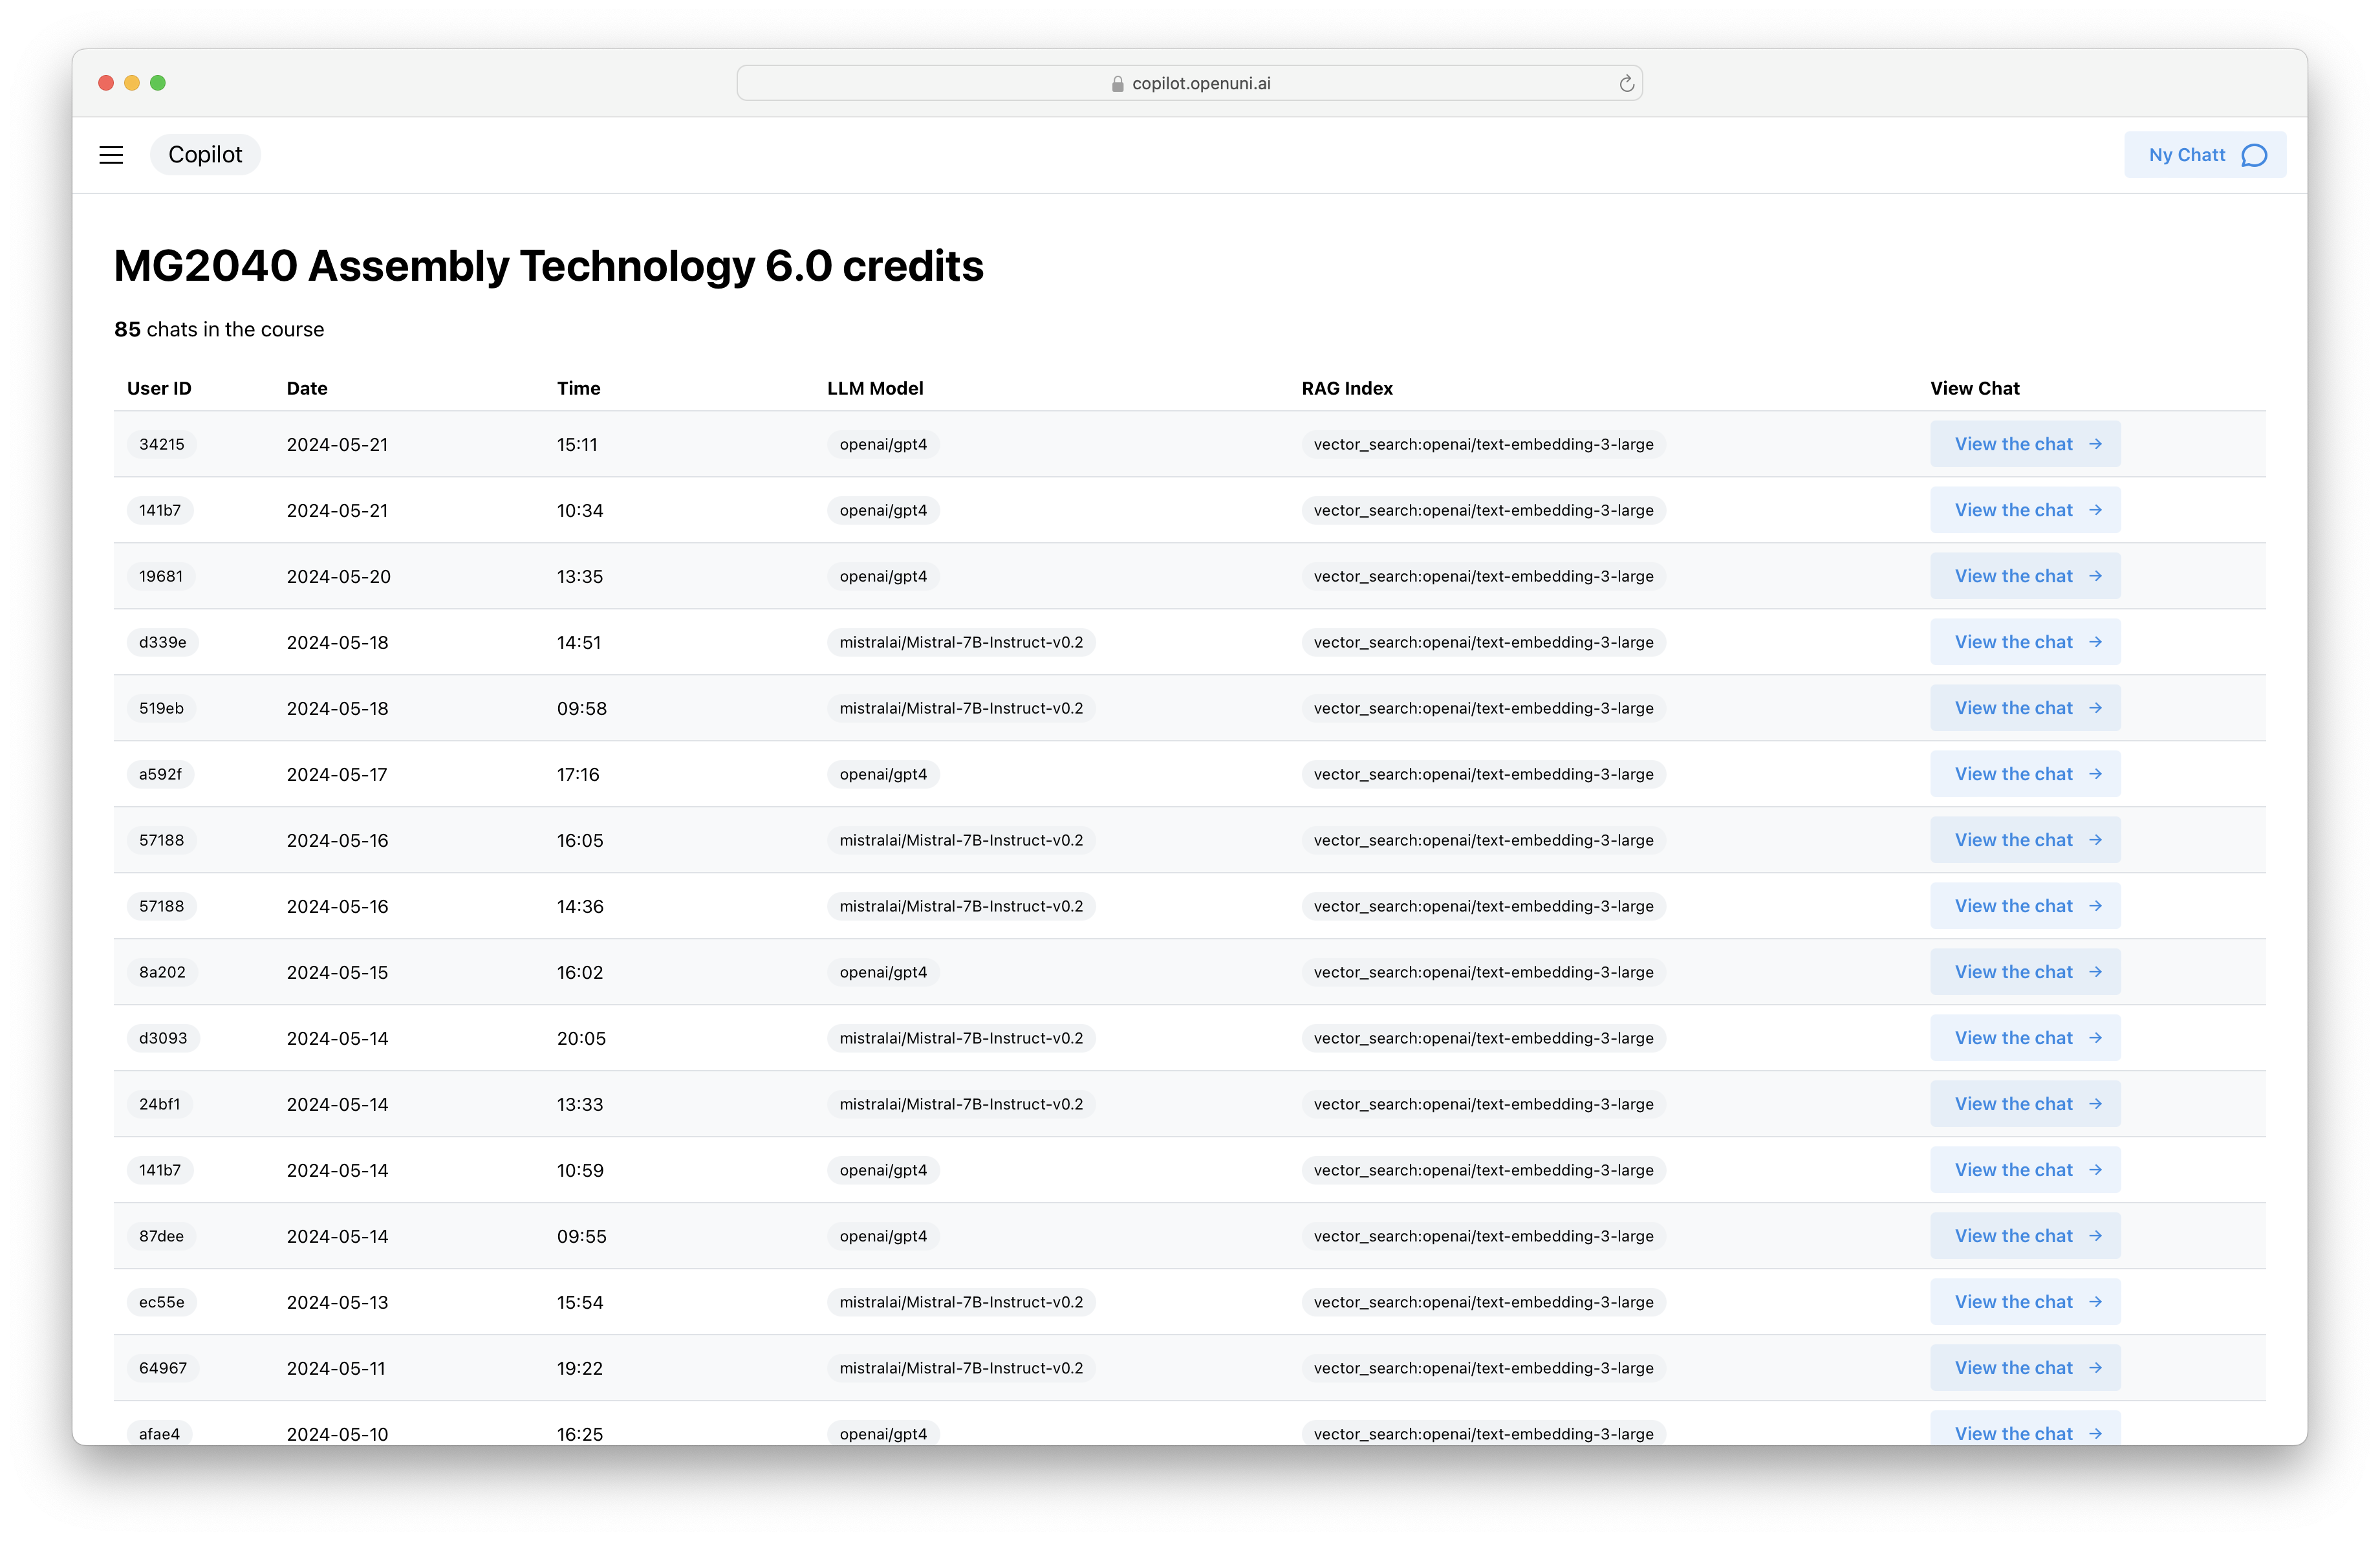
\includegraphics[width=\textwidth]{content/figures/assets/20-list-of-conversations.png}
    \caption{The view available to teachers and TAs that shows all conversations students have had with the assistant}
    \label{fig:list_of_conversations}
\end{figure}



\section{How the software is deployed}


Considering the nature of running \gls{LLM}s at scale the software had quite compute-intensive requirements. Due to sponsorship from KTH Innovation there were credits accessible on Amazon AWS that were available to use for the study. This meant AWS was a suitable cloud infrastructure provider to deploy the software that was built for the study.


AWS has hundreds of services of varying levels of abstraction. The requirements on the infrastructure for this study was primarily that it had to support GPU heavy compute-workloads. Since the software was built to be packed into Docker images, the infrastructure had to support connecting GPU devices to the running Docker containers. AWS \gls{ECS} supports creating \textit{"Task Definitions"} and executing them in services that are hosted on their fully managed \textit{Fargate} platform, or hosting them on regular \gls{EC2}-instances. The latter has a wide array of instance definitions to choose from, of which multiple has one or more GPU devices connected. The \gls{ECS} platform was therefore chosen as the main deployment platform for the software. The entire system architecture can be seen in figure~\ref{fig:aws_diagram}.


% https://lucid.app/lucidchart/4fca3d7e-5905-40a3-8926-917ce384926b/edit

\begin{figure}[H]
    \centering
    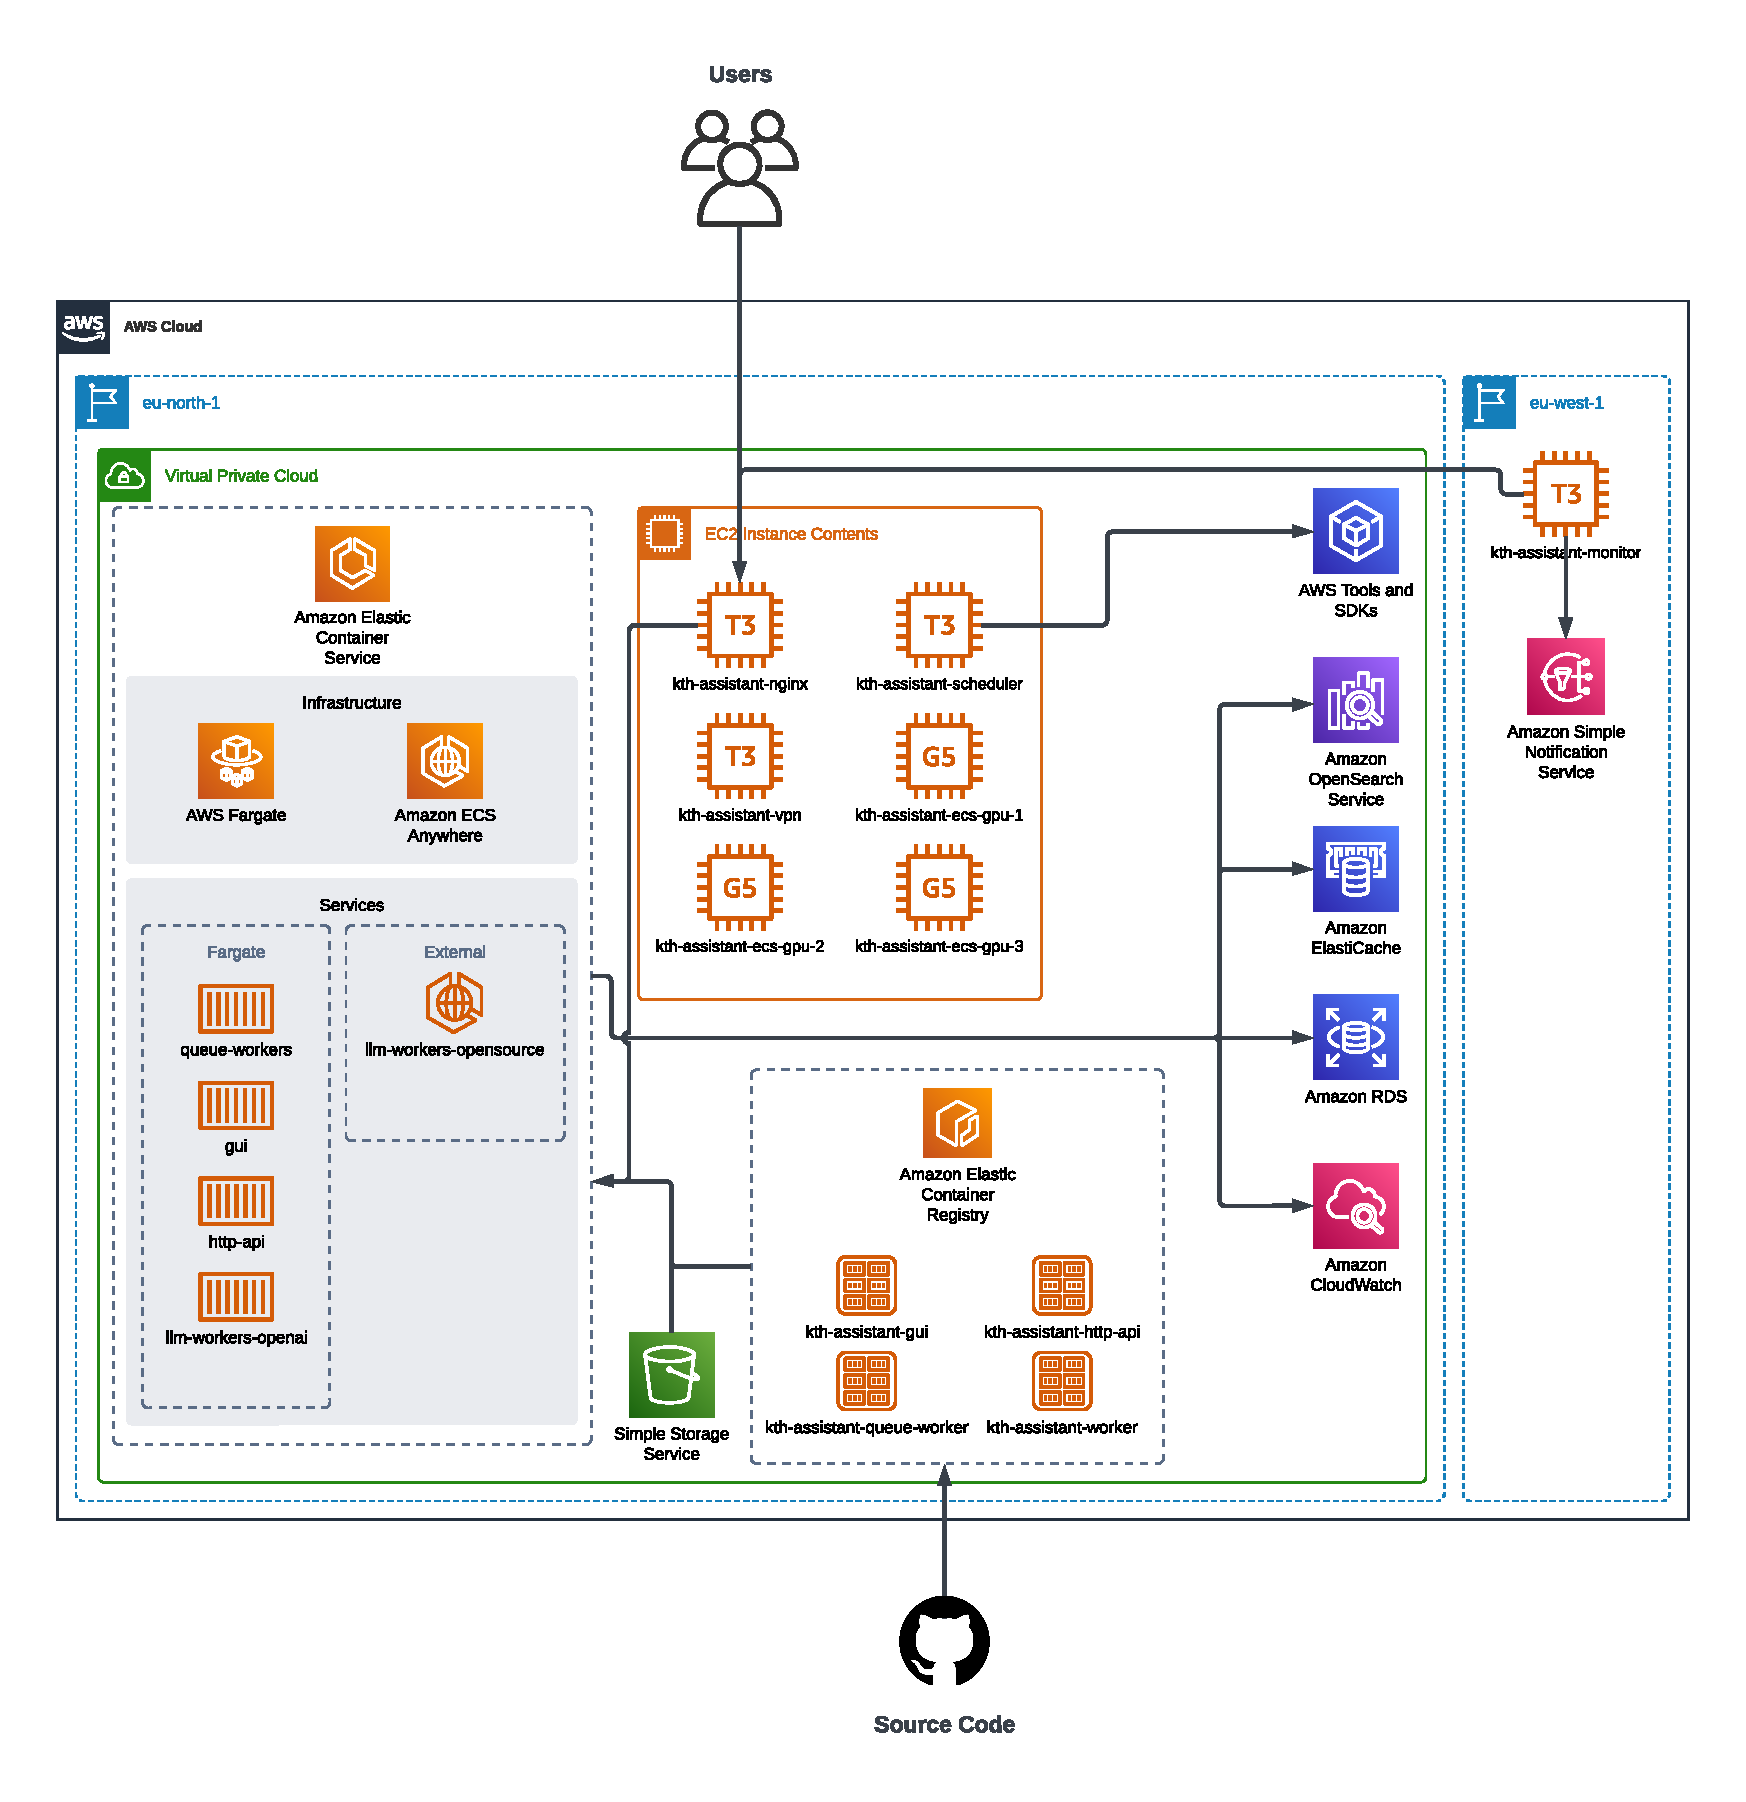
\includegraphics[width=\textwidth]{content/figures/assets/07-aws-diagram.pdf}
    \caption{Diagram that shows how the software was deployed on Amazon AWS}
    \label{fig:aws_diagram}
\end{figure}



In the repository for the source code there are a few github workflows, one of which builds the executables for the project. The executables are four docker images, these are:


\begin{itemize}
        \item \textbf{HTTP API:} This docker image runs the HTTP and Websocket servers for the software.
        \item \textbf{GUI:} This runs a small node server that servers the user interface for the software.
        \item \textbf{LLM Worker:} This runs a worker node for a given \gls{LLM} in the system
        \item \textbf{Queue Worker:} This executes a pool of worker nodes for the jobs that can be dispatched in the system
\end{itemize}


Each of these images are published to their respective \gls{ECR}-registry. The \gls{ECR} are themselves used as source for the task definitions in \gls{ECS}. Together with configuration stored in \gls{S3} the image and task definition are deployed into services in \gls{ECS}. These services can be scaled independently of each other, and use different hosting environments depending on their workload.


Each service can be scaled manually or put in auto scaling groups. The only service that would see any considerable load is the \textit{LLM-worker} containers. However, since they need to keep the \gls{LLM} in-memory in order to provide real time answers to users, it can’t be scaled using traditional metrics such as CPU or memory usage. No sophisticated auto-scaling was configured, since it was deemed unnecessary for this study. Instead, the study relied upon a schedule maintained by a simple script that during certain peak hours scaled up the infrastructure necessary to run more nodes for each enabled \gls{LLM} or embedding function.


Traditional services in AWS were used for running the respective component of the application. One postgres server was deployed in \gls{RDS}, an in-memory Redis cache was created in \textit{Amazon ElastiCache} and an OpenSearch cluster was created in \textit{Amazon OpenSearch Service}. Logs from all services and software components were collected in \textit{Amazon CloudWatch}.


Whilst the service was operational keeping track of whether the system was operational became a priority. During the initial development and deployment it became necessary to track if the service was up and running and be notified of any outages. Therefore a simple playwright script was built that simulated a student entering a question in each course room on a rotating schedule. This would publish a message on a \gls{SNS} topic that would trigger an email if a response couldn’t be produced by the system.




% \sweExpl{Hårdvara / Mjukvarudesign ... / modell / Simuleringsmodell och parametrar / …}




% \sweExpl{Figur~\ref{fig:homepageicon}  visar en enkel ikon för en hemsida. Tiden för att få tillgång till den här sidan när den laddas kommer att kvantifieras i en serie experiment. De konfigurationer som har testats i provbänk listas ini tabell~\ref{tab:configstested}.\\
% Vad du har gjort? Hur gjorde du det? Vilka designval gjorde du?}


% \section{Implementation …/Modeling/Simulation/…}
% \label{sec:implementationDetails}


% \subsection{Some examples of coding}


% \engExpl{This section is simply to show some example of how you can include code in your thesis - this is not a section you would have in your thesis.}
% \sweExpl{Det här avsnittet är helt enkelt för att visa ett exempel på hur du kan inkludera kod i ditt examensarbete - det här är inte ett avsnitt du skulle ha i ditt examensarbete.}


% \subsection{Some examples of figures in tikz}


% \engExpl{This section is simply to show some example of how you can draw your own figures for in your thesis - this is not a section you would have in your thesis.}
% \sweExpl{Det här avsnittet är helt enkelt för att visa ett exempel på hur du kan rita dina egna figurer i ditt examensarbete – det här är inte ett avsnitt du skulle ha i ditt examensarbete.}
% These figures are just some examples to show that you can draw your own figures for in your thesis. This has two advantages: \first you do not have to worry about copyrights -- as these are your own figures and \Second the text is now readable and not simply a picture of text -- so screen readers can read the figure's contents to someone who is listening to the contents of your thesis.


% \subsubsection{Azure's Form Recognizer}


\cleardoublepage